%!TEX TS-program = xelatex

  %%%%%%%%%%%%%%%%%%%%%%%%%%%%%%%%%%%%%%%%%
% The Legrand Orange Book
% LaTeX Template
% Version 1.4 (12/4/14)
%
% This template has been downloaded from:
% http://www.LaTeXTemplates.com
%
% Original author:
% Mathias Legrand (legrand.mathias@gmail.com)
%
% License:
% CC BY-NC-SA 3.0 (http://creativecommons.org/licenses/by-nc-sa/3.0/)
%
% Compiling this template:
% This template uses biber for its bibliography and makeindex for its index.
% When you first open the template, compile it from the command line with the 
% commands below to make sure your LaTeX distribution is configured correctly:
%
% 1) pdflatex main
% 2) makeindex main.idx -s StyleInd.ist
% 3) biber main
% 4) pdflatex main x 2
%
% After this, when you wish to update the bibliography/index use the appropriate
% command above and make sure to compile with pdflatex several times 
% afterwards to propagate your changes to the document.
%
% This template also uses a number of packages which may need to be
% updated to the newest versions for the template to compile. It is strongly
% recommended you update your LaTeX distribution if you have any
% compilation errors.
%
% Important note:
% Chapter heading images should have a 2:1 width:height ratio,
% e.g. 920px width and 460px height.
%
%%%%%%%%%%%%%%%%%%%%%%%%%%%%%%%%%%%%%%%%%

%-=-=-=-=-=-=-=-=-=-=-=-=-=-=-=-=-=-=-=-=-=-=-=-=
%
%	PACKAGES AND OTHER DOCUMENT CONFIGURATIONS
%
%-=-=-=-=-=-=-=-=-=-=-=-=-=-=-=-=-=-=-=-=-=-=-=-=

\documentclass[11pt,fleqn]{book} % Default font size and left-justified equations

\usepackage[top=3cm,bottom=3cm,left=3.2cm,right=3.2cm,headsep=10pt,a4paper]{geometry} % Page margins

\usepackage{xcolor} % Required for specifying colors by name
\definecolor{ocre}{RGB}{0,126,196} % Define the orange color used for highlighting throughout the book
\newcommand{\alert}[1]{{\color{stockholmPink}{#1}}}
\newcommand{\mathref}[1]{{\color{stockholmPurple}{#1}}}

% Define Stockholms Stad Colors
\definecolor{stockholmPink}{RGB}{196,0,104}
% HEX #c40064
\definecolor{stockholmLightPink}{RGB}{254,222,237}
% HEX #fedeed
\definecolor{stockholmGreen}{RGB}{40,157,147}
% HEX #00867f
\definecolor{stockholmLightGreen}{RGB}{182,215,211}
% HEX #d5f7f4
\definecolor{stockholmOrange}{RGB}{203,80,25}
% HEX #dd4a2c
\definecolor{stockholmLightOrange}{RGB}{233,189,155}
% HEX #ffd7d2
\definecolor{stockholmBlue}{RGB}{0,126,196}
% HEX #006ebf
\definecolor{stockholmLightBlue}{RGB}{172,199,233}
% HEX #d6edfc
\definecolor{stockholmPurple}{RGB}{104,55,136}
% HEX #5d237d
\definecolor{stockholmLightPurple}{RGB}{188,170,208}
% HEX #f1e6fc
\definecolor{stockholmYellow}{RGB}{252,191,10}
% HEX #fcbf0a
\definecolor{stockholmGrey}{RGB}{245,243,238}
% HEX #f5f3ee
\definecolor{stockholmDarkGrey}{RGB}{51,51,51}
% HEX #333333

\usepackage{multicol}

%-=-=-=-=-=-=-=-=-=-=-=-=-=-=-=-=-=-=-=-=-=-=-=-=
%	FONT SETTINGS
%-=-=-=-=-=-=-=-=-=-=-=-=-=-=-=-=-=-=-=-=-=-=-=-=

%\usepackage{avant} % Use the Avantgarde font for headings
\usepackage{times} % Use the Times font for headings
\usepackage{mathpazo}
%\usepackage{mathptmx} % Use the Adobe Times Roman as the default text font together with math symbols from the Sym­bol, Chancery and Com­puter Modern fonts
\usepackage{microtype} % Slightly tweak font spacing for aesthetics
\usepackage[utf8]{inputenc} % Required for including letters with accents
\usepackage[T1]{fontenc} % Use 8-bit encoding that has 256 glyphs
\usepackage{xspace} % Used for printing a trailing space better than using a tilde (~) using the \xspace command

%-=-=-=-=-=-=-=-=-=-=-=-=-=-=-=-=-=-=-=-=-=-=-=-=
%	BIBLIOGRAPHY
%-=-=-=-=-=-=-=-=-=-=-=-=-=-=-=-=-=-=-=-=-=-=-=-=
\usepackage[style=alphabetic,sorting=nyt,sortcites=true,autopunct=true,babel=hyphen,hyperref=true,abbreviate=false,backref=true,backend=biber]{biblatex}
\addbibresource{bibliography.bib} % BibTeX bibliography file
\defbibheading{bibempty}{}

%-=-=-=-=-=-=-=-=-=-=-=-=-=-=-=-=-=-=-=-=-=-=-=-=
%	INDEX
%-=-=-=-=-=-=-=-=-=-=-=-=-=-=-=-=-=-=-=-=-=-=-=-=
\usepackage{calc} % For simpler calculation - used for spacing the index letter headings correctly
\usepackage{makeidx} % Required to make an index
\makeindex % Tells LaTeX to create the files required for indexing

%-=-=-=-=-=-=-=-=-=-=-=-=-=-=-=-=-=-=-=-=-=-=-=-=
%	MATHEMATICS SETTINGS
%-=-=-=-=-=-=-=-=-=-=-=-=-=-=-=-=-=-=-=-=-=-=-=-=

\usepackage{
amsmath,
amssymb,
amsfonts,
amsthm,
cancel,
colortbl,
longtable,
pdflscape,
sagetex,
setspace,
mathtools,
pgfplots
}


%-=-=-=-=-=-=-=-=-=-=-=-=-=-=-=-=-=-=-=-=-=-=-=-=
%	TIKZ LIBRARIES
%-=-=-=-=-=-=-=-=-=-=-=-=-=-=-=-=-=-=-=-=-=-=-=-=

%-=-=-=-=-=-=-=-=-=-=-=-=-=-=-=-=-=-=-=-=-=-=-=-=
%	TIKZ LIBRARIES
%-=-=-=-=-=-=-=-=-=-=-=-=-=-=-=-=-=-=-=-=-=-=-=-=

\usetikzlibrary{
arrows,
backgrounds,
fit,
chains,
calc,
decorations.pathmorphing,
matrix,
mindmap,
positioning,
shapes,
shadows,
trees
}

\tikzset{ >=stealth', help lines/.style={dashed, thick}, axis/.style={<->}, important line/.style={thick}, connection/.style={thick, dotted},}

\tikzstyle{firstterm} = [circle, draw, fill=stockholmPink!20, text centered,minimum size=1cm]
\tikzstyle{secondterm} = [circle, draw, fill=stockholmBlue!20, text centered, node distance=0.25cm,minimum size=1cm]
\tikzstyle{terms} = [rectangle, draw, fill=stockholmDarkGrey!20, text centered, node distance=0.25cm,minimum size=1cm]
\tikzstyle{factoradd} = [rectangle, draw=none, fill=white, text centered, node distance=0.25cm,minimum size=1cm]
\tikzstyle{multiply} = [rectangle, draw, fill=stockholmDarkGrey!20, text centered, minimum height=0.75cm,minimum size=1cm]
\tikzstyle{add} = [rectangle, draw, fill=stockholmGreen!20, text centered, minimum height=0.75cm,minimum size=1cm]
\tikzstyle{line} = [draw, color=black!50, -latex']
% Define the style for the red dotted boxes
\tikzset{factordotted/.style={draw=stockholmPurple!50!white, line width=1pt,
                               dash pattern=on 1pt off 4pt on 6pt off 4pt,
                                inner sep=4mm, rectangle, rounded corners}}
%-=-=-=-=-=-=-=-=-=-=-=-=-=-=-=-=-=-=-=-=-=-=-=-=
%	SIMPLIFYING EXPRESSIONS
%-=-=-=-=-=-=-=-=-=-=-=-=-=-=-=-=-=-=-=-=-=-=-=-=

\tikzstyle{operation} = [rectangle, draw, fill=sthlmBlue!40, text centered, rounded corners]
\tikzstyle{function} = [rectangle, draw, fill=sthlmPurple!40, text centered, rounded corners]
\tikzstyle{notation} = [rectangle, draw, fill=sthlmGreen!40, text centered, rounded corners]
\tikzstyle{algorithm} = [rectangle, draw, fill=sthlmOrange!40, text centered, rounded corners]
\tikzstyle{delim} = [rectangle, draw, fill=sthlmYellow!40, text centered, rounded corners]
\tikzstyle{property} = [rectangle, draw, fill=sthlmRed!40, text centered, rounded corners]
\tikzstyle{hide} = [rectangle, draw, fill=sthlmGrey, text centered, rounded corners]
\tikzstyle{active} = [rectangle, draw, fill=sthlmDarkGrey, text=white, text centered, rounded corners]
\tikzstyle{line} = [draw, very thick, color=black!50, -latex']

\tikzset{functiondotted/.style={draw=sthlmPurple!50!white, line width=1pt,
                               dash pattern=on 1pt off 4pt on 6pt off 4pt,
                                inner sep=4mm, rectangle, rounded corners}}
								
\tikzset{productdotted/.style={draw=sthlmBlue!50!white, line width=1pt,
                               dash pattern=on 1pt off 4pt on 6pt off 4pt,
                                inner sep=4mm, rectangle, rounded corners}}
								
\tikzset{sumdotted/.style={draw=sthlmRed!50!white, line width=1pt,
                               dash pattern=on 1pt off 4pt on 6pt off 4pt,
                                inner sep=4mm, rectangle, rounded corners}}


%-=-=-=-=-=-=-=-=-=-=-=-=-=-=-=-=-=-=-=-=-=-=-=-=
%	MATH COMMANDS
%-=-=-=-=-=-=-=-=-=-=-=-=-=-=-=-=-=-=-=-=-=-=-=-=

\newcommand{\unit}[1]{\ensuremath{\, \mathrm{#1}}}
\newcommand{\limit}{\displaystyle\lim}
\newcommand{\impart}{\textrm{Im}}
\newcommand{\repart}{\textrm{Re}}
\newcommand{\integer}{\mathbb{Z}}
\newcommand{\real}{\mathbb{R}}
\newcommand{\degree}{^{\circ}}
\newcommand{\rad}{\unit{rad}}
\newcommand{\dd}{\mathrm{d}}
\newcommand{\dx}{\mathrm{d}x}
\newcommand{\dy}{\mathrm{d}y}
\newcommand{\dr}{\mathrm{d}r}
\newcommand{\dtheta}{\mathrm{d}\theta}
\newcommand{\dydx}{\dfrac{\mathrm{d}y}{\mathrm{d}x}}
\newcommand{\dydt}{\dfrac{\mathrm{d}y}{\mathrm{d}t}}
\newcommand{\dydu}{\dfrac{\mathrm{d}y}{\mathrm{d}u}}
\newcommand{\dudx}{\dfrac{\mathrm{d}u}{\mathrm{d}x}}
\newcommand{\dxdt}{\dfrac{\mathrm{d}x}{\mathrm{d}t}}
\newcommand{\vect}[1]{\boldsymbol{#1}}
\newcommand{\farg}[1]{{\color{stockholmBlue}{\left[\boldsymbol{#1}\right]}}}
\newcommand{\cBlue}[1]{{\color{stockholmBlue}{#1}}}
\newcommand{\cGreen}[1]{{\color{stockholmGreen}{#1}}}
\newcommand{\cYellow}[1]{{\color{stockholmYellow}{#1}}}
\newcommand{\cPurple}[1]{{\color{stockholmPurple}{#1}}}
\newcommand{\cOrange}[1]{{\color{stockholmOrange}{#1}}}
\newcommand{\chide}[1]{{\color{stockholmDarkGrey}{#1}}}
\newcommand{\cGrey}[1]{{\color{stockholmGrey}{#1}}}
\newcommand{\cDarkGrey}[1]{{\color{stockholmDarkGrey}{#1}}}
\newcommand{\cDarkBlue}[1]{{\color{stockholmDarkBlue}{#1}}}
\newcommand{\cLightBlue}[1]{{\color{stockholmLightBlue}{#1}}}
\newcommand{\cRed}[1]{{\color{stockholmPink}{#1}}}
\newcommand{\cLightRed}[1]{{\color{stockholmPink}{#1}}}
\newcommand{\sname}[1]{\texttt{#1}}
\newcommand{\inv}{^{-1}}
\newcommand{\cb}{$\Box$}
\newcommand{\lesssteps}{\cGreen{\textbf{Less Steps Solution:}}}
\newcommand{\solnsteps}{\cGreen{\textbf{Solution:}}}
\newcommand{\qdependlist}{\cDarkGrey{\textbf{Dependencies:}}}
\newcommand{\suchthat}{\;\ifnum\currentgrouptype=16 \middle\fi|\;}
% used in tables
\newcommand{\cellyes}{\cellcolor{stockholmGreen!30}Yes}  
\newcommand{\cellno}{\cellcolor{stockholmPink!30}No}  
\newcommand{\ihat}{\hat{\imath}}
\newcommand{\jhat}{\hat{\jmath}} 
%-=-=-=-=-=-=-=-=-=-=-=-=-=-=-=-=-=-=-=-=-=-=-=-=
%
%	IMPORT STRUCTURE
%
%-=-=-=-=-=-=-=-=-=-=-=-=-=-=-=-=-=-=-=-=-=-=-=-=

%%%%%%%%%%%%%%%%%%%%%%%%%%%%%%%%%%%%%%%%%
% The Legrand Orange Book
% Structural Definitions File
% Version 2.0 (9/2/15)
%
% Original author:
% Mathias Legrand (legrand.mathias@gmail.com) with modifications by:
% Vel (vel@latextemplates.com)
% 
% This file has been downloaded from:
% http://www.LaTeXTemplates.com
%
% License:
% CC BY-NC-SA 3.0 (http://creativecommons.org/licenses/by-nc-sa/3.0/)
%
%%%%%%%%%%%%%%%%%%%%%%%%%%%%%%%%%%%%%%%%%

%----------------------------------------------------------------------------------------
%	VARIOUS REQUIRED PACKAGES AND CONFIGURATIONS
%----------------------------------------------------------------------------------------

\usepackage[top=3cm,bottom=3cm,left=3cm,right=3cm,headsep=10pt,a4paper]{geometry} % Page margins

\usepackage{graphicx} % Required for including pictures
\graphicspath{{Pictures/}} % Specifies the directory where pictures are stored

\usepackage{lipsum} % Inserts dummy text

\usepackage{tikz} % Required for drawing custom shapes

\usepackage[english]{babel} % English language/hyphenation

\usepackage{enumitem} % Customize lists
\setlist{nolistsep} % Reduce spacing between bullet points and numbered lists

\usepackage{booktabs} % Required for nicer horizontal rules in tables

\usepackage{sagetex}

\usepackage{xcolor} % Required for specifying colors by name
\definecolor{ocre}{RGB}{0,126,196} % Define the orange color used for highlighting throughout the book

%-=-=-=-=-=-=-=-=-=-=-=-=-=-=-=-=-=-=-=-=-=-=-=-=
%	MATHEMATICS SETTINGS
%-=-=-=-=-=-=-=-=-=-=-=-=-=-=-=-=-=-=-=-=-=-=-=-=

\usepackage{
amsmath,
amssymb,
amsfonts,
amsthm,
cancel,
colortbl,
longtable,
pdflscape,
setspace,
mathtools,
pgfplots
}
%-=-=-=-=-=-=-=-=-=-=-=-=-=-=-=-=-=-=-=-=-=-=-=-=	
%	sthlm COLOR THEME
%-=-=-=-=-=-=-=-=-=-=-=-=-=-=-=-=-=-=-=-=-=-=-=-=

%== BLUE
	\definecolor{sthlmLightBlue}{RGB}{214,237,252} % HEX #d6edfc
		\newcommand{\csthlmLightBlue}[1]{{\color{sthlmLightBlue}{#1}}}
	\definecolor{sthlmBlue}{RGB}{0,110,191} % HEX #006ebf
		\newcommand{\csthlmBlue}[1]{{\color{sthlmBlue}{#1}}}
	%\definecolor{sthlmDarkBlue}{RGB}{} %HEX #
		%\newcommand{\csthlmDarkBlue}[1]{{\color{sthlmDarkBlue}{#1}}}

%== GREEN

	\definecolor{sthlmLightGreen}{RGB}{213,247,244} % HEX #0d5f7f4
		\newcommand{\csthlmLightGreen}[1]{{\color{sthlmLightGreen}{#1}}}
	\definecolor{sthlmGreen}{RGB}{0,134,127} % #00867f
		\newcommand{\csthlmGreen}[1]{{\color{sthlmGreen}{#1}}}

%== GREY
	%\definecolor{sthlmLightGrey}{RGB}{}
		%\newcommand{\csthlmLightGrey}[1]{{\color{sthlmLightGrey}{#1}}}
	\definecolor{sthlmGrey}{RGB}{245,243,238} % HEX #f5f3ee
		\newcommand{\csthlmGrey}[1]{{\color{sthlmGrey}{#1}}}
	\definecolor{sthlmDarkGrey}{RGB}{51,51,51} % HEX #333333
		\newcommand{\csthlmDarkGrey}[1]{{\color{sthlmDarkGrey}{#1}}} 

%== ORANGE
	\definecolor{sthlmLightOrange}{RGB}{255,215,210} % HEX #ffd7d2
		\newcommand{\csthlmLightOrange}[1]{{\color{sthlmLightOrange}{#1}}}
	\definecolor{sthlmOrange}{RGB}{221,74,44} % HEX #dd4a2c
		\newcommand{\csthlmOrange}[1]{{\color{sthlmOrange}{#1}}}

%== PURPLE	

	\definecolor{sthlmLightPurple}{RGB}{241,230,252} % HEX #f1e6fc
		\newcommand{\csthlmLightPurple}[1]{{\color{sthlmLightPurple}{#1}}}
	\definecolor{sthlmPurple}{RGB}{93,35,125} % HEX #5d237d
		\newcommand{\csthlmPurple}[1]{{\color{sthlmPurple}{#1}}}

%== RED
					
	\definecolor{sthlmLightRed}{RGB}{254,222,237} % HEX #c40064
		\newcommand{\csthlmLightRed}[1]{{\color{sthlmLightRed}{#1}}}
	\definecolor{sthlmRed}{RGB}{196,0,100} % HEX #c40064
		\newcommand{\csthlmRed}[1]{{\color{sthlmRed}{#1}}}
	%\definecolor{sthlmDarkRed}{RGB}{} % HEX #fedeed
		%\newcommand{\csthlmDarkRed}[1]{{\color{sthlmDarkRed}{#1}}}	

%== YELLOW
		
	%\definecolor{sthlmLightYellow}{RGB}{}
		%\newcommand{\csthlmLightYellow}[1]{{\color{sthlmLightYellow}{#1}}}
	\definecolor{sthlmYellow}{RGB}{252,191,10} % HEX #fcbf0a
		\newcommand{\csthlmYellow}[1]{{\color{sthlmYellow}{#1}}}

%-=-=-=-=-=-=-=-=-=-=-=-=-=-=-=-=-=-=-=-=-=-=-=-=	
%	ISSR COLORS
%-=-=-=-=-=-=-=-=-=-=-=-=-=-=-=-=-=-=-=-=-=-=-=-=

%== BLUE
	\definecolor{issrBlue}{RGB}{0,111,174} % HEX #0066cc
		\newcommand{\cissrBlue}[1]{{\color{issrBlue}{#1}}}
		
%== GREY
	\definecolor{issrGrey}{RGB}{167,169,172} % HEX #999999
		\newcommand{\cissrGrey}[1]{{\color{issrGrey}{#1}}}
		
%-=-=-=-=-=-=-=-=-=-=-=-=-=-=-=-=-=-=-=-=-=-=-=-=	
%	GLOBAL COLOR THEME
%-=-=-=-=-=-=-=-=-=-=-=-=-=-=-=-=-=-=-=-=-=-=-=-=

%== BLUE

	\newcommand{\cLightBlue}[1]{{\color{sthlmLightBlue}{#1}}}
	\newcommand{\cBlue}[1]{{\color{sthlmBlue}{#1}}}
	\newcommand{\cDarkBlue}[1]{{\color{sthlmDarkBlue}{#1}}}

%== GREEN

	\newcommand{\cLightGreen}[1]{{\color{}{#1}}}
	\newcommand{\cGreen}[1]{{\color{sthlmGreen}{#1}}}
	\newcommand{\cDarkGreen}[1]{{\color{}{#1}}}

%== GREY

	\newcommand{\cLightGrey}[1]{{\color{sthlmLightGrey}{#1}}}
	\newcommand{\cGrey}[1]{{\color{sthlmGrey}{#1}}}
	\newcommand{\cDarkGrey}[1]{{\color{sthlmDarkGrey}{#1}}}

%== ORANGE

	\newcommand{\cLightOrange}[1]{{\color{}{#1}}}
	\newcommand{\cOrange}[1]{{\color{}{#1}}}
	\newcommand{\cDarkOrange}[1]{{\color{}{#1}}}

%== PURPLE

	\newcommand{\cLightPurple}[1]{{\color{}{#1}}}
	\newcommand{\cPurple}[1]{{\color{sthlmPurple}{#1}}}
	\newcommand{\cDarkPurple}[1]{{\color{}{#1}}}

%== RED

	\newcommand{\cLightRed}[1]{{\color{sthlmLightRed}{#1}}}
	\newcommand{\cRed}[1]{{\color{sthlmRed}{#1}}}
	\newcommand{\cDarkRed}[1]{{\color{sthlmDarkRed}{#1}}}

%== YELLOW

	\newcommand{\cLightYellow}[1]{{\color{sthlmLightYellow}{#1}}}
	\newcommand{\cYellow}[1]{{\color{sthlmYellow}{#1}}}
	\newcommand{\cDarkYellow}[1]{{\color{}{#1}}}
	
\newcommand{\alert}[1]{{\color{sthlmRed}{#1}}}
\newcommand{\mathref}[1]{{\color{sthlmPurple}{#1}}}

\usepackage{multicol}
%----------------------------------------------------------------------------------------
%	FONTS
%----------------------------------------------------------------------------------------

\usepackage{avant} % Use the Avantgarde font for headings
%\usepackage{times} % Use the Times font for headings
\usepackage{mathptmx} % Use the Adobe Times Roman as the default text font together with math symbols from the Sym­bol, Chancery and Com­puter Modern fonts

\usepackage{microtype} % Slightly tweak font spacing for aesthetics
\usepackage[utf8]{inputenc} % Required for including letters with accents
\usepackage[T1]{fontenc} % Use 8-bit encoding that has 256 glyphs

%----------------------------------------------------------------------------------------
%	BIBLIOGRAPHY AND INDEX
%----------------------------------------------------------------------------------------

\usepackage[style=alphabetic,citestyle=numeric,sorting=nyt,sortcites=true,autopunct=true,babel=hyphen,hyperref=true,abbreviate=false,backref=true,backend=biber]{biblatex}
\addbibresource{bibliography.bib} % BibTeX bibliography file
\defbibheading{bibempty}{}

\usepackage{calc} % For simpler calculation - used for spacing the index letter headings correctly
\usepackage{makeidx} % Required to make an index
\makeindex % Tells LaTeX to create the files required for indexing

%----------------------------------------------------------------------------------------
%	MAIN TABLE OF CONTENTS
%----------------------------------------------------------------------------------------

\usepackage{titletoc} % Required for manipulating the table of contents

\contentsmargin{0cm} % Removes the default margin

% Part text styling
\titlecontents{part}[0cm]
{\addvspace{20pt}\centering\large\bfseries}
{}
{}
{}

% Chapter text styling
\titlecontents{chapter}[1.25cm] % Indentation
{\addvspace{12pt}\large\sffamily\bfseries} % Spacing and font options for chapters
{\color{ocre!60}\contentslabel[\Large\thecontentslabel]{1.25cm}\color{ocre}} % Chapter number
{\color{ocre}}  
{\color{ocre!60}\normalsize\;\titlerule*[.5pc]{.}\;\thecontentspage} % Page number

% Section text styling
\titlecontents{section}[1.25cm] % Indentation
{\addvspace{3pt}\sffamily\bfseries} % Spacing and font options for sections
{\contentslabel[\thecontentslabel]{1.25cm}} % Section number
{}
{\hfill\color{black}\thecontentspage} % Page number
[]

% Subsection text styling
\titlecontents{subsection}[1.25cm] % Indentation
{\addvspace{1pt}\sffamily\small} % Spacing and font options for subsections
{\contentslabel[\thecontentslabel]{1.25cm}} % Subsection number
{}
{\ \titlerule*[.5pc]{.}\;\thecontentspage} % Page number
[]

% List of figures
\titlecontents{figure}[0em]
{\addvspace{-5pt}\sffamily}
{\thecontentslabel\hspace*{1em}}
{}
{\ \titlerule*[.5pc]{.}\;\thecontentspage}
[]

% List of tables
\titlecontents{table}[0em]
{\addvspace{-5pt}\sffamily}
{\thecontentslabel\hspace*{1em}}
{}
{\ \titlerule*[.5pc]{.}\;\thecontentspage}
[]

%----------------------------------------------------------------------------------------
%	MINI TABLE OF CONTENTS IN PART HEADS
%----------------------------------------------------------------------------------------

% Chapter text styling
\titlecontents{lchapter}[0em] % Indenting
{\addvspace{15pt}\large\sffamily\bfseries} % Spacing and font options for chapters
{\color{ocre}\contentslabel[\Large\thecontentslabel]{1.25cm}\color{ocre}} % Chapter number
{}  
{\color{ocre}\normalsize\sffamily\bfseries\;\titlerule*[.5pc]{.}\;\thecontentspage} % Page number

% Section text styling
\titlecontents{lsection}[0em] % Indenting
{\sffamily\small} % Spacing and font options for sections
{\contentslabel[\thecontentslabel]{1.25cm}} % Section number
{}
{}

% Subsection text styling
\titlecontents{lsubsection}[.5em] % Indentation
{\normalfont\footnotesize\sffamily} % Font settings
{}
{}
{}

%----------------------------------------------------------------------------------------
%	PAGE HEADERS
%----------------------------------------------------------------------------------------

\usepackage{fancyhdr} % Required for header and footer configuration

\pagestyle{fancy}
\renewcommand{\chaptermark}[1]{\markboth{\sffamily\normalsize\bfseries\chaptername\ \thechapter.\ #1}{}} % Chapter text font settings
\renewcommand{\sectionmark}[1]{\markright{\sffamily\normalsize\thesection\hspace{5pt}#1}{}} % Section text font settings
\fancyhf{} \fancyhead[LE,RO]{\sffamily\normalsize\thepage} % Font setting for the page number in the header
\fancyhead[LO]{\rightmark} % Print the nearest section name on the left side of odd pages
\fancyhead[RE]{\leftmark} % Print the current chapter name on the right side of even pages
\renewcommand{\headrulewidth}{0.5pt} % Width of the rule under the header
\addtolength{\headheight}{2.5pt} % Increase the spacing around the header slightly
\renewcommand{\footrulewidth}{0pt} % Removes the rule in the footer
\fancypagestyle{plain}{\fancyhead{}\renewcommand{\headrulewidth}{0pt}} % Style for when a plain pagestyle is specified

% Removes the header from odd empty pages at the end of chapters
\makeatletter
\renewcommand{\cleardoublepage}{
\clearpage\ifodd\c@page\else
\hbox{}
\vspace*{\fill}
\thispagestyle{empty}
\newpage
\fi}

%----------------------------------------------------------------------------------------
%	THEOREM STYLES
%----------------------------------------------------------------------------------------

\usepackage{amsmath,amsfonts,amssymb,amsthm} % For math equations, theorems, symbols, etc

\newcommand{\intoo}[2]{\mathopen{]}#1\,;#2\mathclose{[}}
\newcommand{\ud}{\mathop{\mathrm{{}d}}\mathopen{}}
\newcommand{\intff}[2]{\mathopen{[}#1\,;#2\mathclose{]}}
\newtheorem{notation}{Notation}[chapter]

\newtheoremstyle{ocrenumbox}% % Theorem style name
{0pt}% Space above
{0pt}% Space below
{\normalfont}% % Body font
{}% Indent amount
{\small\bf\sffamily\color{ocre}}% % Theorem head font
{\;}% Punctuation after theorem head
{0.25em}% Space after theorem head
{\small\sffamily\color{ocre}\thmname{#1}\nobreakspace\thmnumber{\@ifnotempty{#1}{}\@upn{#2}}% Theorem text (e.g. Theorem 2.1)
\thmnote{\nobreakspace\the\thm@notefont\sffamily\bfseries\color{black}---\nobreakspace#3.}} % Optional theorem note
\renewcommand{\qedsymbol}{$\blacksquare$}% Optional qed square

\newtheoremstyle{blacknumexa}% Theorem style Example
{5pt}% Space above
{5pt}% Space below
{\normalfont}% Body font
{} % Indent amount
{\small\bf\sffamily\color{sthlmGreen}}% Theorem head font
{\;}% Punctuation after theorem head
{0.25em}% Space after theorem head
{\nobreakspace\thmname{#1}\nobreakspace\thmnumber{\@ifnotempty{#1}{}\@upn{#2}}% Theorem text (e.g. Theorem 2.1)
\thmnote{\nobreakspace\the\thm@notefont\sffamily\bfseries---\nobreakspace#3.}}% Optional theorem note

\newtheoremstyle{blacknumexe}% Theorem style Exercise
{5pt}% Space above
{5pt}% Space below
{\normalfont}% Body font
{} % Indent amount
{\small\bf\sffamily\color{ocre}}% Theorem head font
{\;}% Punctuation after theorem head
{0.25em}% Space after theorem head
{\nobreakspace\thmname{#1}\nobreakspace\thmnumber{\@ifnotempty{#1}{}\@upn{#2}}% Theorem text (e.g. Theorem 2.1)
\thmnote{\nobreakspace\the\thm@notefont\sffamily\bfseries---\nobreakspace#3.}}% Optional theorem note

\newtheoremstyle{blacknumessential}% Theorem style name
{5pt}% Space above
{5pt}% Space below
{\normalfont}% Body font
{} % Indent amount
{\small\bf\sffamily\color{sthlmRed}}% Theorem head font
{\;}% Punctuation after theorem head
{0.25em}% Space after theorem head
{\nobreakspace\thmname{#1}\nobreakspace\thmnumber{\@ifnotempty{#1}{}\@upn{#2}}% Theorem text (e.g. Theorem 2.1)
\thmnote{\nobreakspace\the\thm@notefont\sffamily\bfseries---\nobreakspace#3.}}% Optional theorem note

\newtheoremstyle{blacknumpro}% Theorem style name properties
{5pt}% Space above
{5pt}% Space below
{\normalfont}% Body font
{} % Indent amount
{\small\bf\sffamily\color{sthlmPurple}}% Theorem head font
{\;}% Punctuation after theorem head
{0.25em}% Space after theorem head
{\nobreakspace\thmname{#1}\nobreakspace\thmnumber{\@ifnotempty{#1}{}\@upn{#2}}% Theorem text (e.g. Theorem 2.1)
\thmnote{\nobreakspace\the\thm@notefont\sffamily\bfseries---\nobreakspace#3.}}% Optional theorem note

\newtheoremstyle{blacknumbox} % Theorem style name
{0pt}% Space above
{0pt}% Space below
{\normalfont}% Body font
{}% Indent amount
{\small\bf\sffamily}% Theorem head font
{\;}% Punctuation after theorem head
{0.25em}% Space after theorem head
{\small\sffamily\thmname{#1}\nobreakspace\thmnumber{\@ifnotempty{#1}{}\@upn{#2}}% Theorem text (e.g. Theorem 2.1)
\thmnote{\nobreakspace\the\thm@notefont\sffamily\bfseries---\nobreakspace#3.}}% Optional theorem note

% Non-boxed/non-framed environments
\newtheoremstyle{ocrenum}% % Theorem style name
{5pt}% Space above
{5pt}% Space below
{\normalfont}% % Body font
{}% Indent amount
{\small\bf\sffamily\color{ocre}}% % Theorem head font
{\;}% Punctuation after theorem head
{0.25em}% Space after theorem head
{\small\sffamily\color{ocre}\thmname{#1}\nobreakspace\thmnumber{\@ifnotempty{#1}{}\@upn{#2}}% Theorem text (e.g. Theorem 2.1)
\thmnote{\nobreakspace\the\thm@notefont\sffamily\bfseries\color{black}---\nobreakspace#3.}} % Optional theorem note
\renewcommand{\qedsymbol}{$\blacksquare$}% Optional qed square
\makeatother

% Defines the theorem text style for each type of theorem to one of the three styles above
\newcounter{dummy} 
\numberwithin{dummy}{section}
\theoremstyle{ocrenumbox}
\newtheorem{theoremeT}[dummy]{Theorem}
\newtheorem{aruleT}[dummy]{Rule}
\newtheorem{definitionT}[dummy]{Definition}
\newtheorem{problem}{Problem}[chapter]
\theoremstyle{blacknumexe}
\newtheorem{exerciseT}{Exercise}[chapter]
\theoremstyle{blacknumexa}
\newtheorem{exampleT}{Example}[chapter]
\theoremstyle{blacknumessential}
\newtheorem{essentialqT}{Essential Questions}[chapter]
\theoremstyle{blacknumpro}
\newtheorem{propertyT}[dummy]{Property}
\theoremstyle{blacknumbox}
\newtheorem{vocabulary}{Vocabulary}[chapter]
%\newtheorem{definitionT}{Definition}[section]
\newtheorem{corollaryT}[dummy]{Corollary}
\theoremstyle{ocrenum}
\newtheorem{proposition}[dummy]{Proposition}

%----------------------------------------------------------------------------------------
%	DEFINITION OF COLORED BOXES
%----------------------------------------------------------------------------------------

\RequirePackage[framemethod=default]{mdframed} % Required for creating the theorem, definition, exercise and corollary boxes

% Theorem box
\newmdenv[skipabove=7pt,
skipbelow=7pt,
backgroundcolor=black!5,
linecolor=ocre,
innerleftmargin=5pt,
innerrightmargin=5pt,
innertopmargin=5pt,
leftmargin=0cm,
rightmargin=0cm,
innerbottommargin=5pt]{tBox}

% Rule box
\newmdenv[skipabove=7pt,
skipbelow=7pt,
backgroundcolor=black!5,
linecolor=ocre,
innerleftmargin=5pt,
innerrightmargin=5pt,
innertopmargin=5pt,
leftmargin=0cm,
rightmargin=0cm,
innerbottommargin=5pt]{arBox}

% Definition box
\newmdenv[skipabove=7pt,
skipbelow=7pt,
backgroundcolor=sthlmDarkGrey!5,
linecolor=ocre,
innerleftmargin=5pt,
innerrightmargin=5pt,
innertopmargin=5pt,
leftmargin=0cm,
rightmargin=0cm,
innerbottommargin=5pt]{dBox}

% Property box
\newmdenv[skipabove=7pt,
skipbelow=7pt,
backgroundcolor=sthlmDarkGrey!5,
linecolor=sthlmPurple,
innerleftmargin=5pt,
innerrightmargin=5pt,
innertopmargin=5pt,
leftmargin=0cm,
rightmargin=0cm,
innerbottommargin=5pt]{prBox}

% Exercise box	  
\newmdenv[skipabove=7pt,
skipbelow=7pt,
rightline=false,
leftline=true,
topline=false,
bottomline=false,
backgroundcolor=ocre!5,
linecolor=ocre,
innerleftmargin=5pt,
innerrightmargin=5pt,
innertopmargin=5pt,
innerbottommargin=5pt,
leftmargin=0cm,
rightmargin=0cm,
linewidth=4pt]{eBox}	

% Definition box
%\newmdenv[skipabove=7pt,
%skipbelow=7pt,
%rightline=false,
%leftline=true,
%topline=false,
%bottomline=false,
%linecolor=ocre,
%innerleftmargin=5pt,
%innerrightmargin=5pt,
%innertopmargin=0pt,
%leftmargin=0cm,
%rightmargin=0cm,
%linewidth=4pt,
%innerbottommargin=0pt]{dBox}

% Example box
\newmdenv[skipabove=7pt,
skipbelow=7pt,
rightline=false,
leftline=true,
topline=false,
bottomline=false,
backgroundcolor=sthlmGreen!5,
linecolor=sthlmGreen,
innerleftmargin=5pt,
innerrightmargin=5pt,
innertopmargin=5pt,
innerbottommargin=5pt,
leftmargin=0cm,
rightmargin=0cm,
linewidth=4pt]{exaBox}

% Essential Question box
\newmdenv[skipabove=7pt,
skipbelow=7pt,
rightline=false,
leftline=false,
topline=true,
bottomline=true,
backgroundcolor=sthlmRed!5,
linecolor=sthlmRed,
innerleftmargin=5pt,
innerrightmargin=5pt,
innertopmargin=5pt,
innerbottommargin=5pt,
leftmargin=0cm,
rightmargin=0cm,
linewidth=4pt]{essentialqBox}			

% Corollary box
\newmdenv[skipabove=7pt,
skipbelow=7pt,
rightline=false,
leftline=true,
topline=false,
bottomline=false,
linecolor=gray,
backgroundcolor=black!5,
innerleftmargin=5pt,
innerrightmargin=5pt,
innertopmargin=5pt,
leftmargin=0cm,
rightmargin=0cm,
linewidth=4pt,
innerbottommargin=5pt]{cBox}

% Creates an environment for each type of theorem and assigns it a theorem text style from the "Theorem Styles" section above and a colored box from above
\newenvironment{theorem}{\begin{tBox}\begin{theoremeT}}{\end{theoremeT}\end{tBox}}
\newenvironment{arule}{\begin{arBox}\begin{aruleT}}{\end{aruleT}\end{arBox}}
\newenvironment{exercise}{\begin{eBox}\begin{exerciseT}}{\hfill{\color{ocre}\tiny\ensuremath{\blacksquare}}\end{exerciseT}\end{eBox}}
\newenvironment{definition}{\begin{dBox}\begin{definitionT}}{\end{definitionT}\end{dBox}}
\newenvironment{property}{\begin{prBox}\begin{propertyT}}{\end{propertyT}\end{prBox}}			  
%\newenvironment{definition}{\begin{dBox}\begin{definitionT}}{\end{definitionT}\end{dBox}}
%\newenvironment{example}{\begin{exBox}\begin{exampleT}}{\end{exampleT}\end{exBox}}	
\newenvironment{example}{\begin{exaBox}\begin{exampleT}}{\hfill{\color{sthlmGreen}\tiny\ensuremath{\blacksquare}}\end{exampleT}\end{exaBox}}
\newenvironment{essentialq}{\begin{essentialqBox}\begin{essentialqT}}{\end{essentialqT}\end{essentialqBox}}
%\newenvironment{example}{\begin{exampleT}}{\hfill{\tiny\ensuremath{\blacksquare}}\end{exampleT}}		
\newenvironment{corollary}{\begin{cBox}\begin{corollaryT}}{\end{corollaryT}\end{cBox}}	

%----------------------------------------------------------------------------------------
%	REMARK ENVIRONMENT
%----------------------------------------------------------------------------------------

\newenvironment{remark}{\par\vspace{10pt}\small % Vertical white space above the remark and smaller font size
\begin{list}{}{
\leftmargin=35pt % Indentation on the left
\rightmargin=25pt}\item\ignorespaces % Indentation on the right
\makebox[-2.5pt]{\begin{tikzpicture}[overlay]
\node[draw=ocre!60,line width=1pt,circle,fill=ocre!25,font=\sffamily\bfseries,inner sep=2pt,outer sep=0pt] at (-15pt,0pt){\textcolor{ocre}{R}};\end{tikzpicture}} % Orange R in a circle
\advance\baselineskip -1pt}{\end{list}\vskip5pt} % Tighter line spacing and white space after remark

\newcommand{\soln}[1]{\par\vspace{10pt}\makebox[15pt]{\begin{tikzpicture}[overlay]
\node[draw=sthlmGreen!70,line width=1pt,circle,fill=sthlmGreen!25,font=\sffamily\bfseries,inner sep=2pt,outer sep=0pt] at (-15pt,0pt){\textcolor{sthlmGreen}{S}};\end{tikzpicture}}\cGreen{\noindent\hrulefill\vskip 15pt}}

%\newcommand{\soln}[1]{\vskip10pt\cGreen{\textbf{Solution:}\hspace{5pt}\noindent\hrulefill \vskip10pt}}

\newcommand{\qdepend}[1]{\par\vspace{10pt}\makebox[15pt]{\begin{tikzpicture}[overlay]
\node[draw=sthlmDarkGrey!70,line width=1pt,circle,fill=sthlmDarkGrey!25,font=\sffamily\bfseries,inner sep=2pt,outer sep=0pt] at (-15pt,0pt){\textcolor{sthlmDarkGrey}{D}};\end{tikzpicture}}\cDarkGrey{\noindent\hrulefill\vskip 15pt}}


%\newenvironment{depend}{\par\vspace{10pt}\small % Vertical white space above the remark and smaller font size
%\begin{list}{}{
%\leftmargin=35pt % Indentation on the left
%\rightmargin=25pt}\item\ignorespaces % Indentation on the right
%\makebox[-2.5pt]{\begin{tikzpicture}[overlay]
%\node[draw=sthlmDarkGrey!60,line width=1pt,circle,fill=sthlmDarkGrey!25,font=\sffamily\bfseries,inner sep=2pt,outer sep=0pt] at (-15pt,0pt){\textcolor{sthlmDarkGrey}{D}};\end{tikzpicture}} % Orange R in a circle
%\advance\baselineskip -1pt}{\end{list}\vskip5pt} % Tighter line spacing and white space after remark


%\newenvironment{soln}{\par\vspace{10pt}\small % Vertical white space above the remark and smaller font size
%\begin{list}{}{
%\leftmargin=35pt % Indentation on the left
%\rightmargin=25pt}\item\ignorespaces % Indentation on the right
%\makebox[-2.5pt]{\begin{tikzpicture}[overlay]
%\node[draw=sthlmGreen!60,line width=1pt,circle,fill=sthlmGreen!25,font=\sffamily\bfseries,inner sep=2pt,outer sep=0pt] at (-15pt,0pt){\textcolor{sthlmGreen}{S}};\end{tikzpicture}}\cGreen{\noindent\hrulefill} % Orange R in a circle
%\advance\baselineskip -1pt}{\end{list}\vskip5pt} % Tighter line spacing and white space after remark

%----------------------------------------------------------------------------------------
%	SECTION NUMBERING IN THE MARGIN
%----------------------------------------------------------------------------------------

\makeatletter
\renewcommand{\@seccntformat}[1]{\llap{\textcolor{ocre}{\csname the#1\endcsname}\hspace{1em}}}                    
\renewcommand{\section}{\@startsection{section}{1}{\z@}
{-4ex \@plus -1ex \@minus -.4ex}
{1ex \@plus.2ex }
{\normalfont\large\sffamily\bfseries}}
\renewcommand{\subsection}{\@startsection {subsection}{2}{\z@}
{-3ex \@plus -0.1ex \@minus -.4ex}
{0.5ex \@plus.2ex }
{\normalfont\sffamily\bfseries}}
\renewcommand{\subsubsection}{\@startsection {subsubsection}{3}{\z@}
{-2ex \@plus -0.1ex \@minus -.2ex}
{.2ex \@plus.2ex }
{\normalfont\small\sffamily\bfseries}}                        
\renewcommand\paragraph{\@startsection{paragraph}{4}{\z@}
{-2ex \@plus-.2ex \@minus .2ex}
{.1ex}
{\normalfont\small\sffamily\bfseries}}

%----------------------------------------------------------------------------------------
%	PART HEADINGS
%----------------------------------------------------------------------------------------

% numbered part in the table of contents
\newcommand{\@mypartnumtocformat}[2]{%
\setlength\fboxsep{0pt}%
\noindent\colorbox{ocre!20}{\strut\parbox[c][.7cm]{\ecart}{\color{ocre!70}\Large\sffamily\bfseries\centering#1}}\hskip\esp\colorbox{ocre!40}{\strut\parbox[c][.7cm]{\linewidth-\ecart-\esp}{\Large\sffamily\centering#2}}}%
%%%%%%%%%%%%%%%%%%%%%%%%%%%%%%%%%%
% unnumbered part in the table of contents
\newcommand{\@myparttocformat}[1]{%
\setlength\fboxsep{0pt}%
\noindent\colorbox{ocre!40}{\strut\parbox[c][.7cm]{\linewidth}{\Large\sffamily\centering#1}}}%
%%%%%%%%%%%%%%%%%%%%%%%%%%%%%%%%%%
\newlength\esp
\setlength\esp{4pt}
\newlength\ecart
\setlength\ecart{1.2cm-\esp}
\newcommand{\thepartimage}{}%
\newcommand{\partimage}[1]{\renewcommand{\thepartimage}{#1}}%
\def\@part[#1]#2{%
\ifnum \c@secnumdepth >-2\relax%
\refstepcounter{part}%
\addcontentsline{toc}{part}{\texorpdfstring{\protect\@mypartnumtocformat{\thepart}{#1}}{\partname~\thepart\ ---\ #1}}
\else%
\addcontentsline{toc}{part}{\texorpdfstring{\protect\@myparttocformat{#1}}{#1}}%
\fi%
\startcontents%
\markboth{}{}%
{\thispagestyle{empty}%
\begin{tikzpicture}[remember picture,overlay]%
\node at (current page.north west){\begin{tikzpicture}[remember picture,overlay]%	
\fill[ocre!20](0cm,0cm) rectangle (\paperwidth,-\paperheight);
\node[anchor=north] at (4cm,-3.25cm){\color{ocre!40}\fontsize{220}{100}\sffamily\bfseries\@Roman\c@part}; 
\node[anchor=south east] at (\paperwidth-1cm,-\paperheight+1cm){\parbox[t][][t]{8.5cm}{
\printcontents{l}{0}{\setcounter{tocdepth}{1}}%
}};
\node[anchor=north east] at (\paperwidth-1.5cm,-3.25cm){\parbox[t][][t]{15cm}{\strut\raggedleft\color{white}\fontsize{30}{30}\sffamily\bfseries#2}};
\end{tikzpicture}};
\end{tikzpicture}}%
\@endpart}
\def\@spart#1{%
\startcontents%
\phantomsection
{\thispagestyle{empty}%
\begin{tikzpicture}[remember picture,overlay]%
\node at (current page.north west){\begin{tikzpicture}[remember picture,overlay]%	
\fill[ocre!20](0cm,0cm) rectangle (\paperwidth,-\paperheight);
\node[anchor=north east] at (\paperwidth-1.5cm,-3.25cm){\parbox[t][][t]{15cm}{\strut\raggedleft\color{white}\fontsize{30}{30}\sffamily\bfseries#1}};
\end{tikzpicture}};
\end{tikzpicture}}
\addcontentsline{toc}{part}{\texorpdfstring{%
\setlength\fboxsep{0pt}%
\noindent\protect\colorbox{ocre!40}{\strut\protect\parbox[c][.7cm]{\linewidth}{\Large\sffamily\protect\centering #1\quad\mbox{}}}}{#1}}%
\@endpart}
\def\@endpart{\vfil\newpage
\if@twoside
\if@openright
\null
\thispagestyle{empty}%
\newpage
\fi
\fi
\if@tempswa
\twocolumn
\fi}

%----------------------------------------------------------------------------------------
%	CHAPTER HEADINGS
%----------------------------------------------------------------------------------------

\newcommand{\thechapterimage}{}%
\newcommand{\chapterimage}[1]{\renewcommand{\thechapterimage}{#1}}%
\def\@makechapterhead#1{%
{\parindent \z@ \raggedright \normalfont
\ifnum \c@secnumdepth >\m@ne
\if@mainmatter
\begin{tikzpicture}[remember picture,overlay]
\node at (current page.north west)
{\begin{tikzpicture}[remember picture,overlay]
\node[anchor=north west,inner sep=0pt] at (0,0) {\includegraphics[width=\paperwidth]{\thechapterimage}};
\draw[anchor=west] (\Gm@lmargin,-9cm) node [line width=2pt,rounded corners=15pt,draw=ocre,fill=white,fill opacity=0.5,inner sep=15pt]{\strut\makebox[22cm]{}};
\draw[anchor=west] (\Gm@lmargin+.3cm,-9cm) node {\huge\sffamily\bfseries\color{black}\thechapter. #1\strut};
\end{tikzpicture}};
\end{tikzpicture}
\else
\begin{tikzpicture}[remember picture,overlay]
\node at (current page.north west)
{\begin{tikzpicture}[remember picture,overlay]
\node[anchor=north west,inner sep=0pt] at (0,0) {\includegraphics[width=\paperwidth]{\thechapterimage}};
\draw[anchor=west] (\Gm@lmargin,-9cm) node [line width=2pt,rounded corners=15pt,draw=ocre,fill=white,fill opacity=0.5,inner sep=15pt]{\strut\makebox[22cm]{}};
\draw[anchor=west] (\Gm@lmargin+.3cm,-9cm) node {\huge\sffamily\bfseries\color{black}#1\strut};
\end{tikzpicture}};
\end{tikzpicture}
\fi\fi\par\vspace*{270\p@}}}

%-------------------------------------------

\def\@makeschapterhead#1{%
\begin{tikzpicture}[remember picture,overlay]
\node at (current page.north west)
{\begin{tikzpicture}[remember picture,overlay]
\node[anchor=north west,inner sep=0pt] at (0,0) {\includegraphics[width=\paperwidth]{\thechapterimage}};
\draw[anchor=west] (\Gm@lmargin,-9cm) node [line width=2pt,rounded corners=15pt,draw=ocre,fill=white,fill opacity=0.5,inner sep=15pt]{\strut\makebox[22cm]{}};
\draw[anchor=west] (\Gm@lmargin+.3cm,-9cm) node {\huge\sffamily\bfseries\color{black}#1\strut};
\end{tikzpicture}};
\end{tikzpicture}
\par\vspace*{270\p@}}
\makeatother

%----------------------------------------------------------------------------------------
%	HYPERLINKS IN THE DOCUMENTS
%----------------------------------------------------------------------------------------

\usepackage{hyperref}
\hypersetup{hidelinks,backref=true,pagebackref=true,hyperindex=true,colorlinks=false,breaklinks=true,urlcolor= ocre,bookmarks=true,bookmarksopen=false,pdftitle={Title},pdfauthor={Author}}
\usepackage{bookmark}
\bookmarksetup{
open,
numbered,
addtohook={%
\ifnum\bookmarkget{level}=0 % chapter
\bookmarksetup{bold}%
\fi
\ifnum\bookmarkget{level}=-1 % part
\bookmarksetup{color=ocre,bold}%
\fi
}
} % Insert the commands.tex file which contains the majority of the structure behind the template

\begin{document}

%-=-=-=-=-=-=-=-=-=-=-=-=-=-=-=-=-=-=-=-=-=-=-=-=
%
%	TITLE PAGE
%
%-=-=-=-=-=-=-=-=-=-=-=-=-=-=-=-=-=-=-=-=-=-=-=-=

\begingroup
\thispagestyle{empty}
\AddToShipoutPicture*{\put(6,5){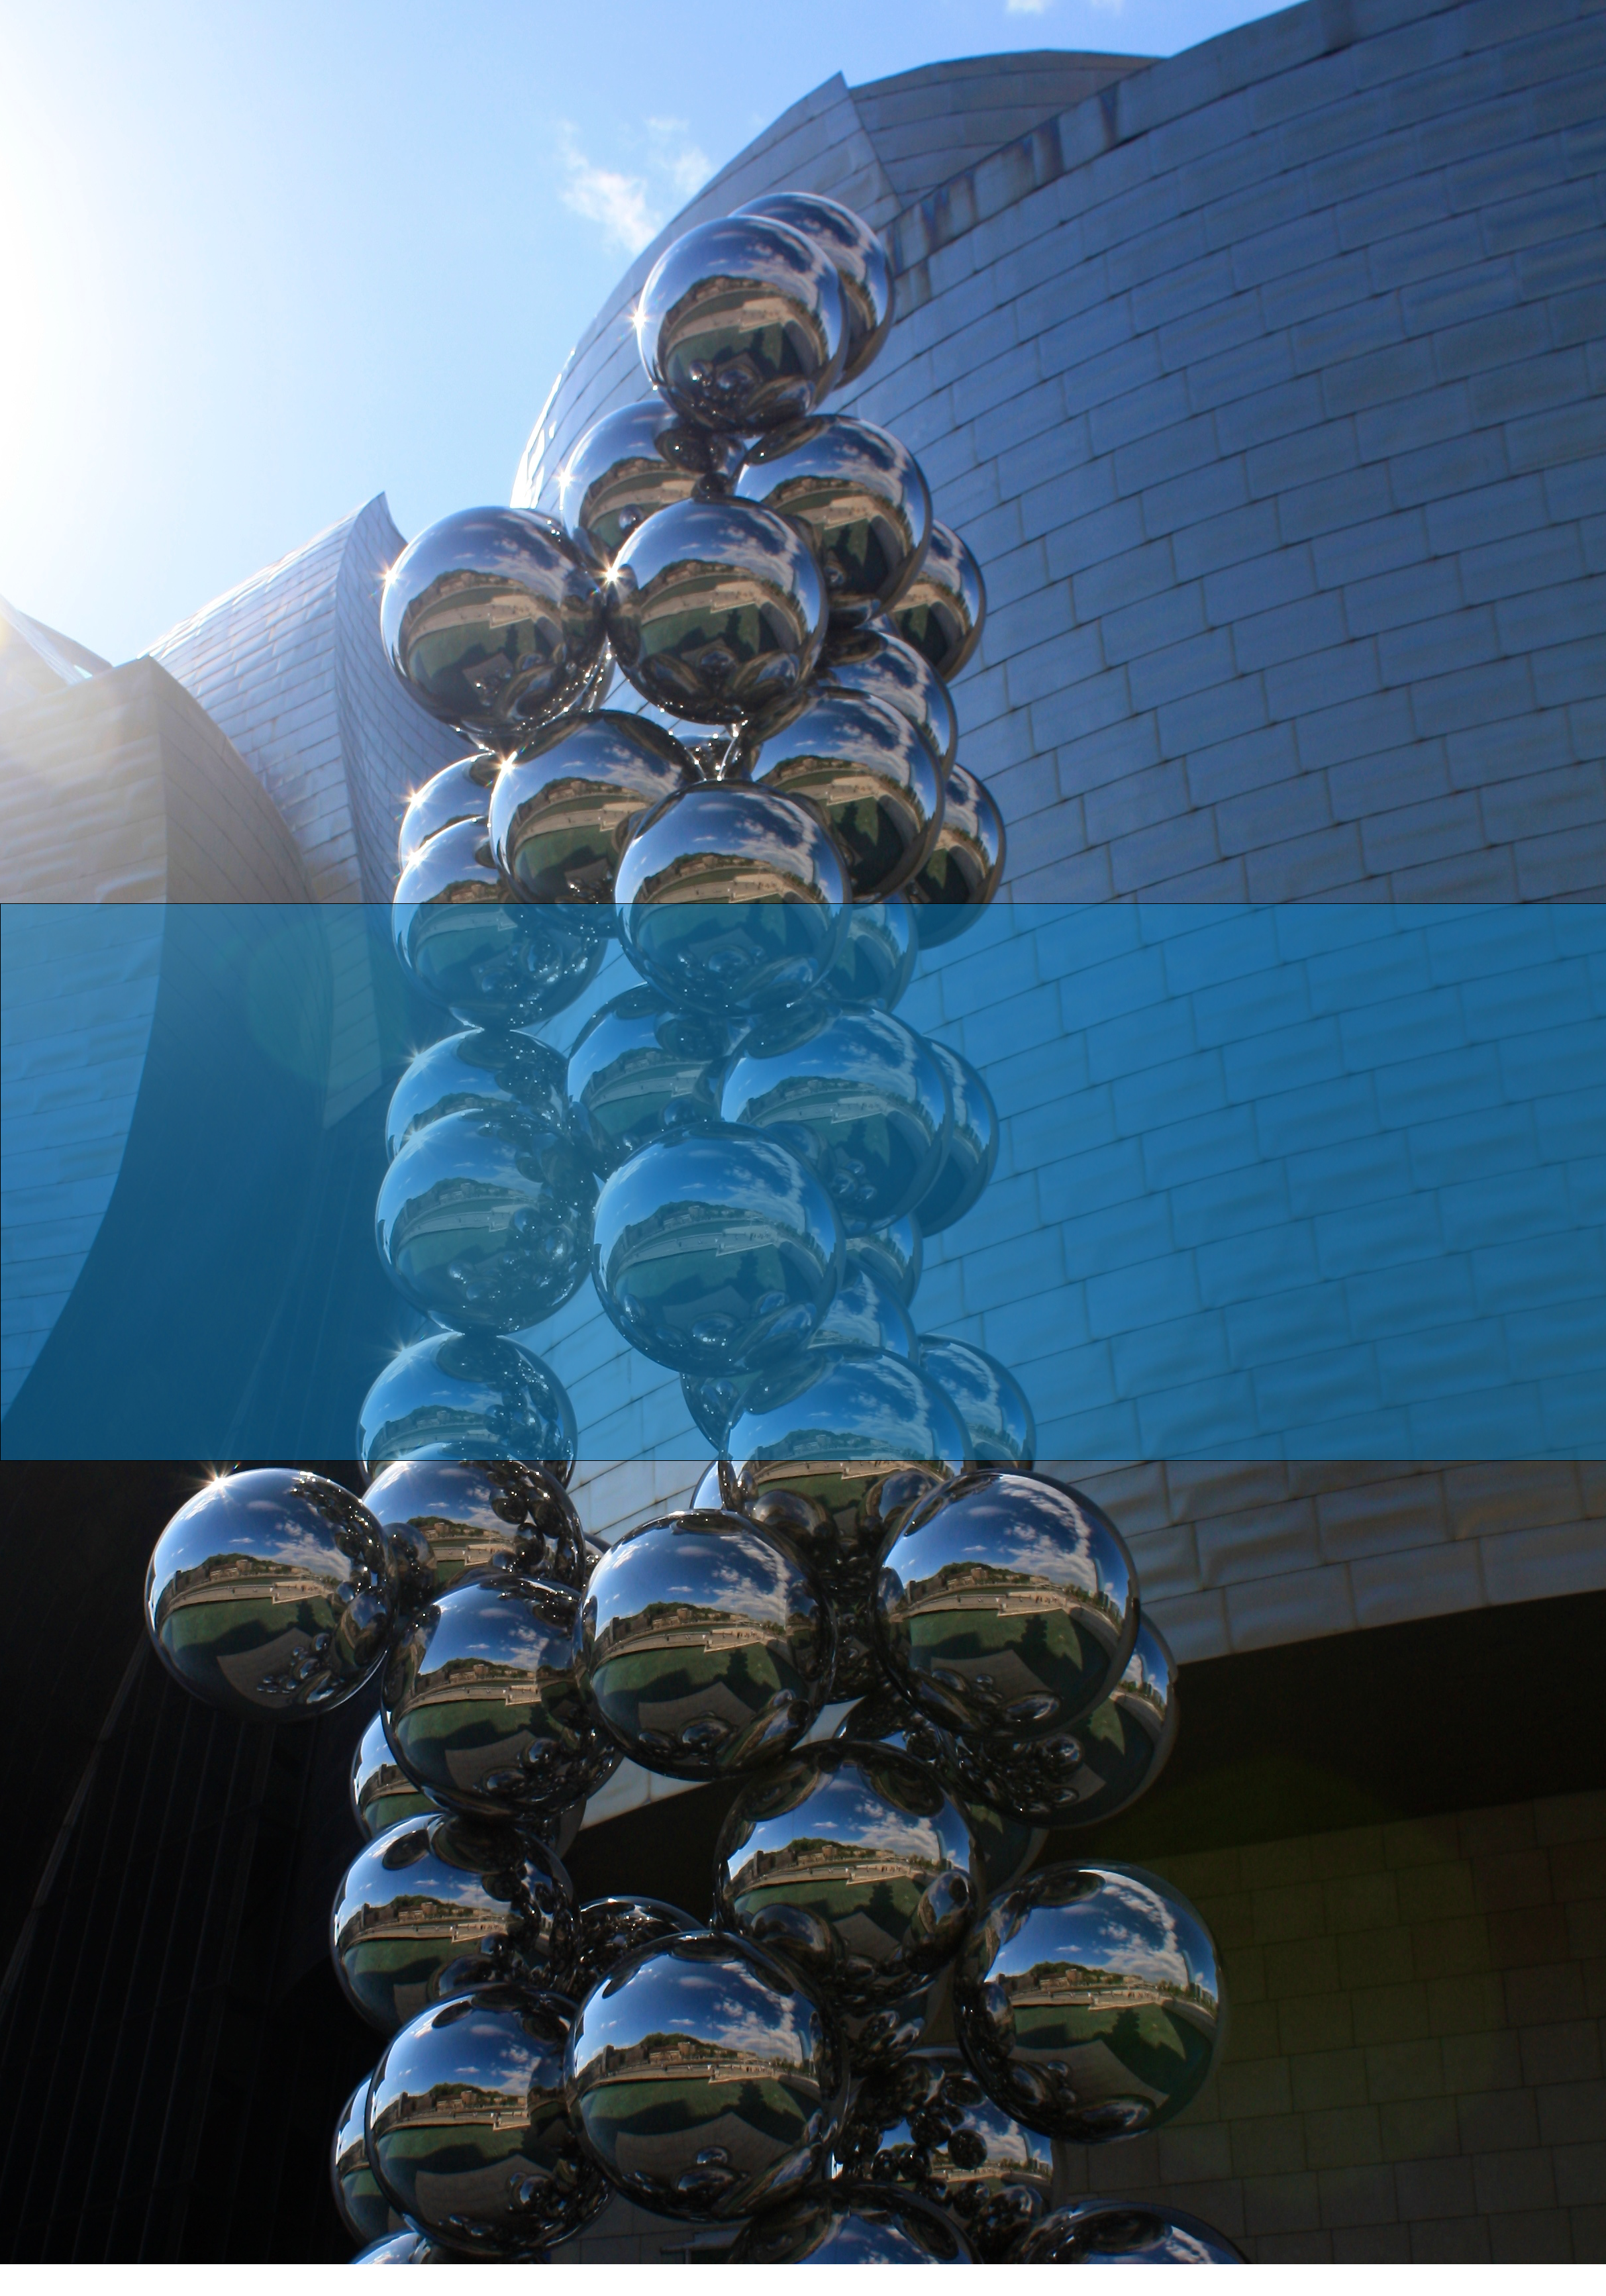
\includegraphics[scale=1]{Pictures/background}}} % Image background
\centering
\vspace*{9cm}
\par\normalfont\fontsize{35}{35}\sffamily\selectfont
{\textcolor{stockholmGrey}{Mathematics Notebook}} \par % Book title
\vspace*{1cm}
{\Huge {\color{stockholmGrey}{Mark H. Olson}}}\par % Author name
\vspace*{1cm}
{\Large {\color{stockholmGrey}{Updated: \today}}}\par % Author name
\endgroup

%%-=-=-=-=-=-=-=-=-=-=-=-=-=-=-=-=-=-=-=-=-=-=-=-=
%
%	COPYRIGHT PAGE
%
%-=-=-=-=-=-=-=-=-=-=-=-=-=-=-=-=-=-=-=-=-=-=-=-=

\newpage
~\vfill
\thispagestyle{empty}

\noindent Copyright \copyright\ 2014 Mark Hendry Olson\\ % Copyright notice

\noindent \textsc{Published by Mark Hendry Olson}\\ % Publisher

\noindent \textsc{hendryolson.com}\\ % URL

\noindent Licensed under the Creative Commons Attribution-NonCommercial 3.0 Unported License (the ``License''). You may not use this file except in compliance with the License. You may obtain a copy of the License at \url{http://creativecommons.org/licenses/by-nc/3.0}. Unless required by applicable law or agreed to in writing, software distributed under the License is distributed on an \textsc{``as is'' basis, without warranties or conditions of any kind}, either express or implied. See the License for the specific language governing permissions and limitations under the License.\\ % License information

\noindent \textit{First printing, March 2013} % Printing/edition date

%-=-=-=-=-=-=-=-=-=-=-=-=-=-=-=-=-=-=-=-=-=-=-=-=
%
%	TABLE OF CONTENTS
%
%-=-=-=-=-=-=-=-=-=-=-=-=-=-=-=-=-=-=-=-=-=-=-=-=

\chapterimage{chapter_head_1.pdf} % Table of contents heading image

\pagestyle{empty} % No headers

\tableofcontents % Print the table of contents itself

\cleardoublepage % Forces the first chapter to start on an odd page so it's on the right

\pagestyle{fancy} % Print headers again

\begin{sagesilent}
var('x')
#t=ZZ.random_element(999999)
t=2015
set_random_seed(t)

# =-=-=-=-=-=-=-=-=-=-=-=-=-=-=
# Question 20141120-211843
# =-=-=-=-=-=-=-=-=-=-=-=-=-=-=

a_20141120_211843=[(ZZ.random_element(2,14)) for i in range(13)]
b_20141120_211843=[(ZZ.random_element(2,14)) for i in range(13)]

for j in range(len(a_20141120_211843)):
  while a_20141120_211843[j]==a_20141120_211843[(j-1)]:
    a_20141120_211843[j]=ZZ.random_element(2,14)

# =-=-=-=-=-=-=-=-=-=-=-=-=-=-=
# Question 20141121-195608
# =-=-=-=-=-=-=-=-=-=-=-=-=-=-=
	
a_20141121_195608=[(ZZ.random_element(2,14)) for i in range(8)]
b_20141121_195608=[(ZZ.random_element(2,14)) for i in range(8)]

for j in range(len(a_20141121_195608)):
  while b_20141121_195608[j]==b_20141121_195608[(j-1)]:
    b_20141121_195608[j]=ZZ.random_element(2,14)
	
for k_20141121_195608 in range(len(a_20141121_195608)):
  while a_20141121_195608[k_20141121_195608]==b_20141121_195608[(k_20141121_195608-1)]:
    a_20141121_195608[k_20141121_195608]=ZZ.random_element(2,14)	

# =-=-=-=-=-=-=-=-=-=-=-=-=-=-=
# Question 20141121-191224
# =-=-=-=-=-=-=-=-=-=-=-=-=-=-=

a_20141121_191224=[(ZZ.random_element(2,14)) for i in range(13)]
b_20141121_191224=[(ZZ.random_element(2,14)) for i in range(13)]

for j in range(len(a_20141121_191224)):
  while a_20141121_191224[j]==a_20141121_191224[(j-1)]:
    a_20141121_191224[j]=ZZ.random_element(2,14)
	
# =-=-=-=-=-=-=-=-=-=-=-=-=-=-=
# Question 20141123-091420
# =-=-=-=-=-=-=-=-=-=-=-=-=-=-=

a_20141123_091420=[(-1)^(ZZ.random_element(1,3))*(ZZ.random_element(2,14)) for i in range(13)]
b_20141123_091420=[(-1)^(ZZ.random_element(1,3))*(ZZ.random_element(2,14)) for i in range(13)]
c_20141123_091420=[(-1)^(ZZ.random_element(1,3))*(ZZ.random_element(2,14)) for i in range(13)]

for j in range(len(a_20141123_091420)):
  while a_20141123_091420[j]==a_20141123_091420[(j-1)]:
    a_20141123_091420[j]=(-1)^(ZZ.random_element(1,3))*(ZZ.random_element(2,14))
\end{sagesilent}
%%-=-=-=-=-=-=-=-=-=-=-=-=-=-=-=-=-=-=-=-=-=-=-=-=
%
%	CHAPTER 
%
%-=-=-=-=-=-=-=-=-=-=-=-=-=-=-=-=-=-=-=-=-=-=-=-=

\chapterimage{chapter_head_2.pdf} % Chapter heading image

\chapter{Arithmetic Expressions}
%!TEX root = /Users/markholson/Dropbox/+Projects/LatexFiles/MathNotebook/20150312-163541-rs2.2N-MarksMathNotebook.tex
%-=-=-=-=-=-=-=-=-=-=-=-=-=-=-=-=-=-=-=-=-=-=-=-=
%
%	CHAPTER 
%
%-=-=-=-=-=-=-=-=-=-=-=-=-=-=-=-=-=-=-=-=-=-=-=-=

\chapterimage{chapter_head_2.pdf} % Chapter heading image

\chapter{Algebraic Expressions}

%-=-=-=-=-=-=-=-=-=-=-=-=-=-=-=-=-=-=-=-=-=-=-=-=
%	SECTION: OPERATION OF ADDITION
%-=-=-=-=-=-=-=-=-=-=-=-=-=-=-=-=-=-=-=-=-=-=-=-=
\section{Expressions}\index{Algebraic Expressions}

\begin{essentialq}\hfill \\

\begin{enumerate}
	\item What is an algebraic expression?
\end{enumerate}

\end{essentialq}


\begin{table}
\begin{tabular}{|l|c|c|c|c|c|c}
\hline
 									& Arithmetic 	& Polynomial	& Algebraic  	\\
\hline
Constant 							& \cellyes		& \cellyes 		& \cellyes		\\
\hline
Factorial 							& \cellyes 		& \cellyes 		& \cellyes		\\
\hline
Variable: parameter/coefficient 	& \cellyes 		& \cellyes 		& \cellyes		\\
\hline
Variable: unknown/indeterminate 	& \cellno 		& \cellyes 		& \cellyes		\\
\hline
Power with $\integer^{+}$ exponent 	& \cellno 		& \cellyes 		& \cellyes		 \\
\hline
Power with $\integer$ exponent 		& \cellno 		& \cellno 		& \cellyes		 \\
\hline
$n$-th root 						& \cellno 		& \cellno 		& \cellyes		\\
\hline
Power with $\mathbb{Q}$ exponent 	& \cellno 		& \cellno 		& \cellyes		 \\
\hline
\end{tabular}
\caption{Names of different types of expressions}\label{tab:tableofexpressions}
\end{table}


%-=-=-= DEFINITION
%\begin{definition}[Algebraic Expression]\index{Algebraic Expression}

%An algebraic expression is made up of one or more terms (operation of addition), which are themselves made up of factors (operation of multiplication).\\

%Algebraic expressions have three different types of multiplicative factors:\\

%\begin{enumerate}   
%	\item constant (coefficient) 
%	\begin{itemize}
%		\item real number 
%		\item parameter 
%	\end{itemize}
%	\item variable
%	\item rational power
%\end{enumerate}
%\hfill \cite{mathworld:algebraicexpression}
%\end{definition}

\section{Polynomial Expressions}\index{Polynomial Expressions}

%-=-=-= DEFINITION
\begin{definition}[Operation of Addition (OOA)]\index{Operation!Operation of Addition}
\begin{align}
\underbrace{\underbrace{a}_{\text{Augend}}+\underbrace{b}_{\text{Addend}}}_{\text{Sum}} \label{eq:ooa}
\end{align}
\end{definition}


%-=-=-= DEFINITION
\begin{definition}[Common Denominator (CD)]\index{Common Denominator}
\begin{subequations}
\begin{align}
\dfrac{a}{b} + \dfrac{c}{b} &= \dfrac{a+c}{b} \label{eq:cd1} \\
\dfrac{a+c}{b}&= \dfrac{a}{b} + \dfrac{c}{b} \label{eq:cd2}
\end{align}
\end{subequations}
\end{definition}

%-=-=-= RULE
\begin{arule}[Fraction Operation of Addition (FOOA)]\index{Fraction Operation of Addition}
\begin{subequations}
\begin{align}
\dfrac{a}{b} + \dfrac{c}{d} &= \dfrac{ad+bc}{bd} \label{eq:fooa1} \\
\dfrac{ad+bc}{bd} &= \dfrac{a}{b} + \dfrac{c}{d} \label{eq:fooa2}
\end{align}
\end{subequations}
\end{arule}

\newpage
\begin{figure}
\begin{tikzpicture}[scale=1, node distance=1.1cm, text width=5em, auto]
    % Place nodes
\node [property] (MId1) {MId};
\node [notation, below of=MId1] (ONeg1) {ONeg};
\node [operation, below of=ONeg1] (DOS1) {DOS};
\node [delim, below of=DOS1] (DELIM) {DELIM};
\node [property, below of=DELIM] (DPE) {DPE};
\node [notation, below of=DPE] (JTC) {JTC};
\node [property, below of=JTC] (CPM) {CPM};
\node [operation, below of=CPM] (OOM) {OOM};
\node [property, right of=OOM, node distance=2.8cm] (APM) {APM};
\node [algorithm, below of=OOM] (RF1) {RF};
\node [algorithm, below of=RF1] (CTJ) {CTJ};
\node [notation, below of=CTJ] (CPA) {CPA};
\node [property, below of=CPA] (DPF) {DPF};
\node [operation, below of=DPF] (OOA) {OOA};
\node [property, right of=OOA,node distance=2.8cm] (APA) {APA};
\node [algorithm, below of=OOA] (RF2) {RF};
\node [property, below of=RF2] (AId) {AId};
\node [operation, below of=AId] (DOS2) {DOS};
\node [notation, below of=DOS2] (ONeg2) {ONeg};
\node [property, below of=ONeg2] (MId2) {MId};

\path [line] (MId1) -- (ONeg1);
\path [line] (ONeg1) -- (DOS1);
\path [line] (DOS1) -- (DELIM);
\path [line] (DELIM) -- (DPE);
\path [line] (DPE) -- (JTC);
\path [line] (JTC) -- (CPM);
\path [line] (CPM) edge [out= 315, in= 150] (APM);
\path [line] (APM) -- (OOM);
\path [line] (OOM) -- (RF1);
\path [line] (RF1) -- (CTJ);
\path [line] (CTJ) -- (CPA);
\path [line] (CPA) -- (DPF);
\path [line] (DPF) edge [out= 315, in= 150] (APA);
\path [line] (APA) -- (OOA);
\path [line] (OOA) -- (RF2);
\path [line] (RF2) -- (AId);
\path [line] (AId) -- (DOS2);
\path [line] (DOS2) -- (ONeg2);
\path [line] (ONeg2) -- (MId2);

\node [function, right of=DELIM, node distance=8cm] (PoTF) {PoTF};
\node [function, below of=PoTF] (RTPo) {RTPo};
\node [function, below of=RTPo] (PoNE1) {PoNE};
\node [function, below of=PoNE1] (PoPr) {PoPr};
\node [function, below of=PoPr] (PoQ) {PoQ};
\node [function, below of=PoQ] (PoPrPo) {PoPrPo};
\node [function, below of=PoPrPo] (PoQPo) {PoQPo};
\node [function, below of=PoQPo] (PrCBPo) {PrCBPo};
\node [function, below of=PrCBPo] (QCBPo) {QCBPo};
\node [function, below of=QCBPo] (PoPo) {PoPo};
\node [function, below of=PoPo] (PoNE2) {PoNE};
\node [operation, below of=PoNE2] (OOE) {OOE};
\node [function, below of=OOE] (PoTR) {PoTR};


\path [line] (DELIM) edge [bend left=30] (PoTF);
\path [line] (PoTF) -- (RTPo);
\path [line] (RTPo) -- (PoNE1);
\path [line] (PoPr) -- (PoQ);
\path [line] (PoQ) -- (PoPrPo);
\path [line] (PoPrPo) -- (PoQPo);
\path [line] (PoQPo) -- (PrCBPo);
\path [line] (PrCBPo) -- (QCBPo);
\path [line] (QCBPo) -- (PoPo);
\path [line] (PoPo) -- (PoNE2);
\path [line] (PoNE2) -- (OOE);
\path [line] (OOE) -- (PoTR);

%\node[productdotted, fit =(DELIM)(JTC)(CPM)(OOM)(RF1)(CTJ)(APM)](product) {};
%\node[left of =product, text centered,](powers) {\textcolor{sthlmPurple}{\textbf{Multiplication}}};
%\node[sumdotted, fit =(CPA)(DPF)(OOA)(RF2)(AId)(ONeg2)(DOS2)(MId2)(APA)](sum2) {};
%\node[sumdotted, fit =(MId1)(ONeg1)(DOS1)](sum1) {};
%\node[left of =sum1, text centered,](powers) {\textcolor{sthlmPurple}{\textbf{Addition}}};
%\node[left of =sum2, text centered,](powers) {\textcolor{sthlmPurple}{\textbf{Addition}}};


\node[functiondotted, fit =(PoTF)(RTPo)(PoNE1)(PoPr)(PoQ)(PoPrPo)(PoQPo)(PrCBPo)(QCBPo)(PoPo)(PoNE2)(OOE)(PoTR)](powerfunctions) {};
\node[below of =PoTR, text centered,](powers) {\textcolor{sthlmPurple}{\textbf{Powers}}};

\path [line] (PoNE1) edge [out= 180, in= 0] (DELIM);

\path [line] (CPM) edge [out= 0, in= 180] (PoPr);

\path [line] (PoTR) edge [out= 180, in= 0] (APM);

\path [line] (AId) edge [out= 180, in= 180] (DELIM);

\end{tikzpicture}
\caption{Simplifying Expressions Workflow: \newline {\color{stockholmPink!40}\ensuremath{\blacksquare}} Property, {\color{stockholmBlue!40}\ensuremath{\blacksquare}} Operation, {\color{stockholmGreen!40}\ensuremath{\blacksquare}} Notation, {\color{stockholmPurple!40}\ensuremath{\blacksquare}} Powers, {\color{stockholmYellow!40}\ensuremath{\blacksquare}} Delimiters, {\color{stockholmOrange!40}\ensuremath{\blacksquare}} Process, {\color{stockholmDarkGrey!40}\ensuremath{\blacksquare}} Not Used}
\end{figure}


%-=-=-= DEFINITION
\begin{definition}[Operation of Multiplication (OOM)] \index{Operation!Operation of Multiplication}
\begin{align}
\underbrace{\underbrace{a}_{\text{Multiplicand}} \cdot \underbrace{b}_{\text{Multiplier}}}_{\text{Product}} \label{eq:oom}
\end{align}
\end{definition}



%-=-=-= DEFINITION
\begin{definition}[Operation of Exponentiation (OOE)]\index{Operation!Operation of Exponentiation}
\begin{align}
\underbrace{{\underbrace{b}_{base}}^{\overbrace{m}^{Exponent}}}_{Power} \label{eq:ooe}
\end{align}
\end{definition}


%-=-=-=-=-=-=-=-=-=-=-=-=-=-=-=-=-=-=-=-=-=-=-=-=
%	SECTION: ALGEBRAIC EXPRESSIONS
%-=-=-=-=-=-=-=-=-=-=-=-=-=-=-=-=-=-=-=-=-=-=-=-=






%-=-=-= DEFINITION
\begin{definition}[Juxtaposition to Center-Dot (JTC)]\index{Notation!Juxtapostion to Center-Dot}
\begin{align}
ab &= a \cdot b \label{eq:jtc}
\end{align}
\end{definition}

%-=-=-= DEFINITION
\begin{definition}[Center-Dot to Justapostion (CTJ)]\index{Notation!Center-Dot to Juxtaposition}
\begin{align}
a \cdot b &= ab \label{eq:ctj}
\end{align}
\end{definition}


%-=-=-= DEFINITION
\begin{definition}[Commutative Property of Multiplication (CPM)]\index{Property!Commutative Property of Multiplication}
\begin{align}
\alert{a} \cdot b &= b \cdot \alert{a} \label{eq:cpm}
\end{align}
\end{definition}



%-=-=-= DEFINITION
\begin{definition}[Multiplicative Inverse (MI)]\index{Multiplicative Inverse}
\begin{subequations}
\begin{align}
a \cdot \alert{\dfrac{1}{a}} &= 1 \label{eq:mi1} \\
a \cdot \alert{a^{-1}} &= 1 \label{eq:mi2} 
\end{align}
\end{subequations}
\end{definition}

%-=-=-= DEFINITION
\begin{definition}[Associative Property of Multiplication (APM)]\index{Property!Associative Property of Multiplication}
\begin{subequations}
\begin{align}
a\cdot b\cdot c &= (a\cdot b)\cdot c \label{eq:apm1} \\
a\cdot b\cdot c &= a\cdot (b\cdot c) \label{eq:apm2}
\end{align}
\end{subequations}
\end{definition}


%-=-=-=-=-=-=-=-=-=-=-=-=-=-=-=-=-=-=-=-=-=-=-=-=
%	SECTION: Powers
%-=-=-=-=-=-=-=-=-=-=-=-=-=-=-=-=-=-=-=-=-=-=-=-=

\subsubsection{Powers}\index{Powers}


\begin{arule}[Power of a Quotient of Powers (PoQPo)]\index{Powers!Power of a Quotient of Powers}
\begin{subequations}
\begin{align}
	\left(\dfrac{a^m}{b^n}\right)^k &= \dfrac{a^{m \cdot k}}{b^{n\cdot k}} \label{eq:poqpo1}\\
	\dfrac{a^{m \cdot k}}{b^{n\cdot k}} &= \left(\dfrac{a^m}{b^n}\right)^k \label{eq:poqpo2}
\end{align}
\end{subequations}
\end{arule}

\begin{arule}[Power of a Product of Powers (PoPrPo)]\index{Powers!Power of a Product of Powers}
\begin{subequations}
\begin{align}
	\left(a^m \cdot b^n\right)^k &= a^{m \cdot k} \cdot b^{n\cdot k} \label{eq:poprpo1}\\
	a^{m \cdot k} \cdot b^{n \cdot k} &= \left(a^m \cdot b^n\right)^k \label{eq:poprpo2}
\end{align}
\end{subequations}
\end{arule}

\begin{definition}[Power To Factor (PoTF)]\index{Powers!Power to Factor}
\begin{align}
a^{\alert{n}} &= a_1 \cdot a_2 \cdot \ldots \cdot a_{n-1} \cdot a_{\alert{n}} \label{eq:potf} 
\end{align}
\end{definition}

\begin{definition}[Factor To Power (FTPo)]\index{Powers!Factor to Power}
\begin{align}
a_1 \cdot a_2 \cdot \ldots \cdot a_{n-1} \cdot a_{\alert{n}} &= a^{\alert{n}} \label{eq:ftpo} 
\end{align}
\end{definition}

%-=-=-= DEFINITION
\begin{definition}[Power Inverse (PoI)]\index{Power Inverse}
\begin{subequations}
\begin{align}
\left(b^{m}\right)^{\frac{1}{m}} &= b  \label{eq:poi} 
\end{align}
\end{subequations}
\end{definition}

%-=-=-= DEFINITION
\begin{definition}[Power Inverse (PoId)]\index{Power Identity}
\begin{subequations}
\begin{align}
1&= b^0  \label{eq:poid1} \\
b^{0}&= 1  \label{eq:poid2} 
\end{align}
\end{subequations}
\end{definition}

\begin{notation}[Radical To Power (RTPo)]\index{Powers!Radical to Power}
\begin{align}
\sqrt[m]{b^n} &= b^{\frac{n}{m}}	 \label{eq:rtpo} 
\end{align}
\end{notation}

\begin{notation}[Power To Radical (PoTR)]\index{Powers!Power to Radical}
\begin{align}
b^{\frac{n}{m}} &= \sqrt[m]{b^n}	 \label{eq:potr} 
\end{align}
\end{notation}




%-=-=-=-=-=-=-=-=-=-=-=-=-=-=-=-=-=-=-=-=-=-=-=-=
%	SUBSECTION: Monomials of Like Terms
%-=-=-=-=-=-=-=-=-=-=-=-=-=-=-=-=-=-=-=-=-=-=-=-=

\subsection{Monomials of Like Terms}\index{Monomials of Like Terms}








%-=-=-= DEFINITION
\begin{definition}[Additive Inverse (AI)]\index{Additive Inverse}
\begin{subequations}
\begin{align}
a + \alert{(-a)} &= 0 \label{eq:ai}
\end{align}
\end{subequations}
\end{definition}




\subsection{Surds}\index{Surds}

%-=-=-= EXAMPLE
\begin{example}[id:20141108-085327] \label{20141108-085327} \index{Example!20141108-085327} \hfill \\

Simplify $2\sqrt{2}-\dfrac{\left(\sqrt{2}\right)^3}{3}-\left(2\left(-\sqrt{2}\right)-\dfrac{\left(-\sqrt{2}\right)^3}{3} \right)$

\soln

\solnsteps
\begin{align*}
2 \sqrt{2}- \dfrac{\alert{1}\left(\alert{1}\sqrt{2}\right)^{3}}{3}-\alert{1} \left(2 \left(-\alert{1}\sqrt{2} \right) - \dfrac{\alert{1} \left(-\alert{1} \sqrt{2}\right)^{3}}{3} \right) && \text{MId} \eqref{eq:mid1} \\
2 \sqrt{2} - \dfrac{1 \left(1\sqrt{2}\right)^{3}}{3}-1 \left(2 \left(\alert{\neg 1} \sqrt{2} \right) - \dfrac{1 \left(\alert{\neg 1} \sqrt{2}\right)^{3}}{3} \right) && \text{ONeg} \eqref{eq:oneg1} \\
2 \sqrt{2} + \dfrac{\neg 1 \left(1\sqrt{2}\right)^{3}}{3}+ \neg 1 \left(2 \left(\alert{\neg 1} \sqrt{2} \right) + \dfrac{\neg 1 \left(\alert{\neg 1} \sqrt{2}\right)^{3}}{3} \right) && \text{DOS} \eqref{eq:dos1} \\
2 \cdot \alert{2^{1/2}} + \dfrac{\neg 1 \left(1 \cdot \alert{2^{1/2}}\right)^{3}}{3} + \neg 1 \left(2 \left(\neg  1 \cdot \alert{2^{1/2}} \right) + \dfrac{\neg 1 \left(\neg  1  \cdot \alert{2^{1/2}}\right)^{3}}{3} \right) && \text{RTPo} \eqref{eq:rtpo} \\
2 \cdot 2^{1/2} + \dfrac{\neg 1 \left(1 \cdot 2^{1/2}\right)^{3}}{3} + \neg 1 \left(\alert{2 \cdot \neg  1 \cdot 2^{1/2}} + \dfrac{\neg 1 \left(\neg 1  \cdot 2^{1/2}\right)^{3}}{3} \right) && \text{JTC} \eqref{eq:jtc} \\
2 \cdot 2^{1/2} + \dfrac{\neg 1 \cdot \alert{1 \cdot 2^{3/2}}}{3} + \neg 1 \left(2 \cdot \neg  1 \cdot 2^{1/2} + \dfrac{\neg 1 \cdot \alert{\neg 1  \cdot 2^{3/2}}}{3} \right) && \text{PoPrPo} \eqref{eq:poprpo1} \\
2 \cdot 2^{1/2} + \dfrac{\neg 1 \cdot 1 \cdot \alert{2^{2/2} \cdot 2^{1/2}}}{3} + \neg 1 \left(2 \cdot \neg  1 \cdot 2^{1/2} + \dfrac{\neg 1 \cdot \neg 1  \cdot \alert{2^{2/2} \cdot 2^{1/2}}}{3} \right) && \text{PrCBPo} \eqref{eq:prcbpo2} \\
2 \cdot 2^{1/2} + \dfrac{\neg 1 \cdot 1 \cdot \alert{2} \cdot 2^{1/2}}{3} + \neg 1 \left(2 \cdot \neg  1 \cdot 2^{1/2} + \dfrac{\neg 1 \cdot \neg 1  \cdot \alert{2} \cdot 2^{1/2}}{3} \right) && \text{MId} \eqref{eq:mid2} \\
2 \cdot \alert{\sqrt{2}} + \dfrac{\neg 1 \cdot 1 \cdot 2 \cdot \alert{\sqrt{2}}}{3} + \neg 1 \left(2 \cdot \neg  1 \cdot \alert{\sqrt{2}} + \dfrac{\neg 1 \cdot \neg 1  \cdot 2 \cdot \alert{\sqrt{2}}}{3} \right) && \text{PoTR} \eqref{eq:potr} \\
2 \cdot \sqrt{2} + \dfrac{\neg 1 \cdot 1 \cdot 2 \cdot \sqrt{2}}{3} + \alert{\neg 1} \cdot 2 \cdot \neg  1 \cdot \sqrt{2} + \dfrac{\alert{\neg 1} \cdot \neg 1 \cdot \neg 1  \cdot 2 \cdot \sqrt{2}}{3}  && \text{DPE} \eqref{eq:dpe1} \\
2 \cdot \sqrt{2} + \dfrac{\neg 2 \cdot \sqrt{2}}{3} + 2 \cdot \sqrt{2} + \dfrac{\neg 2 \cdot \sqrt{2}}{3}  && \text{OOM} \eqref{eq:oom} \\
2\sqrt{2} + \dfrac{\neg 2\sqrt{2}}{3} + 2\sqrt{2} + \dfrac{\neg 2\sqrt{2}}{3} && \text{CTJ} \eqref{eq:ctj} \\
\left(2 + \dfrac{\neg 2}{3} + 2 + \dfrac{\neg 2}{3} \right)  \sqrt{2} && \text{DPF} \eqref{eq:dpf1} \\
\dfrac{8}{3}\sqrt{2} && \text{OOA} \eqref{eq:ooa} 
\end{align*}

\qdepend 

\qdependlist
example \ref{20141108-083108}-20141108-083108

\end{example}




\include{chapter-univariatepolynomialexpressions}
%!TEX root = /Users/markholson/Dropbox/+Projects/LatexFiles/MathNotebook/20150312-163541-rs2.2N-MarksMathNotebook
%-=-=-=-=-=-=-=-=-=-=-=-=-=-=-=-=-=-=-=-=-=-=-=-=
%
%	CHAPTER 
%
%-=-=-=-=-=-=-=-=-=-=-=-=-=-=-=-=-=-=-=-=-=-=-=-=

\chapterimage{chapter_head_2.pdf} % Chapter heading image

\chapter{Multivariate Polynomial Expressions}

%-=-=-=-=-=-=-=-=-=-=-=-=-=-=-=-=-=-=-=-=-=-=-=-=
%	SECTION: OPERATION OF ADDITION
%-=-=-=-=-=-=-=-=-=-=-=-=-=-=-=-=-=-=-=-=-=-=-=-=
\section*{Classification of Multivariate Polynomial Expressions}\index{Classification of Multivariate Polynomial Expressions}

%-=-=-=-=-=-=-=-=-=-=-=-=-=-=-=-=-=-=-=-=-=-=-=-=
%	SECTION: 
%-=-=-=-=-=-=-=-=-=-=-=-=-=-=-=-=-=-=-=-=-=-=-=-=
\section*{Degree -1 Multivariate Polynomials}\index{Degree -1 Multivariate Polynomials}

%-=-=-=-=-=-=-=-=-=-=-=-=-=-=-=-=
%	SUBSECTION: 
%-=-=-=-=-=-=-=-=-=-=-=-=-=-=-=-=
\subsection*{Monomials}

%-=-=-=-=-=-=-=-=-=-=-=-=-=-=-=-=-=-=-=-=-=-=-=-=
%	SECTION: 
%-=-=-=-=-=-=-=-=-=-=-=-=-=-=-=-=-=-=-=-=-=-=-=-=
\section*{Degree 0 Multivariate Polynomials}\index{Degree 0 Multivariate Polynomials}

%-=-=-=-=-=-=-=-=-=-=-=-=-=-=-=-=
%	SUBSECTION: 
%-=-=-=-=-=-=-=-=-=-=-=-=-=-=-=-=
\subsection*{Monomials}

%-=-=-=-=-=-=-=-=-=-=-=-=-=-=-=-=-=-=-=-=-=-=-=-=
%	SECTION: 
%-=-=-=-=-=-=-=-=-=-=-=-=-=-=-=-=-=-=-=-=-=-=-=-=
\section*{Degree 1 Multivariate Polynomials}\index{Degree 1 Multivariate Polynomials}

%-=-=-=-=-=-=-=-=-=-=-=-=-=-=-=-=
%	SUBSECTION: 
%-=-=-=-=-=-=-=-=-=-=-=-=-=-=-=-=
\subsection*{Monomials}

%-=-=-=-=-=-=-=-=-=-=-=-=-=-=-=-=
%	SUBSECTION: 
%-=-=-=-=-=-=-=-=-=-=-=-=-=-=-=-=
\subsection*{Binomials}

%-=-=-=-=-=-=-=-=-=-=-=-=-=-=-=-=-=-=-=-=-=-=-=-=
%	SECTION: 
%-=-=-=-=-=-=-=-=-=-=-=-=-=-=-=-=-=-=-=-=-=-=-=-=
\section*{Degree 2 Multivariate Polynomials}\index{Degree 2 Multivariate Polynomials}

%-=-=-=-=-=-=-=-=-=-=-=-=-=-=-=-=
%	SUBSECTION: 
%-=-=-=-=-=-=-=-=-=-=-=-=-=-=-=-=
\subsection*{Monomials}

%-=-=-= EXAMPLE
\begin{example}[id:20141106-150953] \label{20141106-150953} \index{Example!20141106-150953} \hfill \\

Simplify $8xy+5xy$

\soln

\solnsteps
\begin{align*}
(8+5)xy && \text{DPF} \eqref{eq:dpf1} \\
13xy && \text{OOA} \eqref{eq:ooa} 
\end{align*}

\soln

\lesssteps
\begin{align*}
13xy && \text{OOA} \eqref{eq:ooa} 
\end{align*}

\end{example}

%-=-=-= EXAMPLE
\begin{example}[id:20141108-193835] \label{20141108-193835} \index{Example!20141108-193835} \hfill \\

Simplify $3xy + 4yx$

\soln

\solnsteps
\begin{align*}
3 \cdot x \cdot y + 4 \cdot y \cdot x && \text{JTC} \eqref{eq:jtc} \\
3 \cdot x \cdot y + 4 \cdot x \cdot y && \text{CPM} \eqref{eq:cpm} \\
3xy+4xy && \text{CTJ} \eqref{eq:ctj} \\
(3+4)xy && \text{DPF} \eqref{eq:dpf1} \\ 
7xy && \text{OOA} \eqref{eq:ooa} 
\end{align*}

\soln

\lesssteps
\begin{align*}
3xy + 4xy && \text{CPM} \eqref{eq:cpm} \\
7xy && \text{OOA} \eqref{eq:ooa} 
\end{align*}

\end{example}


%-=-=-= EXAMPLE
\begin{example}[id:20141108-180100] \label{20141108-180100} \index{Example!20141108-180100} \hfill \\

Simplify $8x \cdot 2y$

\soln

\solnsteps
\begin{align*}
8 \cdot x \cdot 2 \cdot y && \text{JTC} \eqref{eq:jtc} \\
8 \cdot 2 \cdot x \cdot y && \text{CPM} \eqref{eq:cpm} \\
(8 \cdot 2) \cdot x \cdot y && \text{APM} \eqref{eq:apm1} \\
16 \cdot x \cdot y && \text{OOM} \eqref{eq:oom} \\
16 xy && \text{CTJ} \eqref{eq:ctj}  
\end{align*}

\soln

\lesssteps
\begin{align*}
8 \cdot 2 \cdot x \cdot y && \text{CPM} \eqref{eq:cpm} \\
16xy && \text{OOM} \eqref{eq:oom} 
\end{align*}

\end{example}

%-=-=-= EXAMPLE
\begin{example}[id:20141108-180608] \label{20141108-180608} \index{Example!20141108-180608} \hfill \\

Simplify $3x \cdot y$

\soln

\solnsteps
\begin{align*}
3x \cdot 1y && \text{MId} \eqref{eq:mid1} \\
3 \cdot x \cdot 1 \cdot y && \text{JTC} \eqref{eq:jtc} \\
3 \cdot 1 \cdot x \cdot y && \text{CPM} \eqref{eq:cpm} \\
(3 \cdot 1) \cdot x \cdot y && \text{CPM} \eqref{eq:cpm} \\
3 \cdot x \cdot y && \text{OOM} \eqref{eq:oom} \\
3xy && \text{CTJ} \eqref{eq:ctj} 
\end{align*}

\soln

\lesssteps
\begin{align*}
3xy && \text{CTJ} \eqref{eq:ctj}  
\end{align*}

\end{example}

%-=-=-=-=-=-=-=-=-=-=-=-=-=-=-=-=
%	SUBSECTION: 
%-=-=-=-=-=-=-=-=-=-=-=-=-=-=-=-=
\subsection*{Binomials}

%-=-=-= EXAMPLE
\begin{example}[id:20141106-151622] \label{20141106-151622} \index{Example!20141106-151622} \hfill \\

Simplify $5xy^2-3xy$

\soln

\solnsteps
\begin{align*}
5xy^2+\neg 3xy && \text{DOS} \eqref{eq:dos1} \\
(5y+\neg 3)xy && \text{DPF} \eqref{eq:dpf1} \\
(5y-3)xy && \text{DOS} \eqref{eq:dos2} 
\end{align*}

\soln

\lesssteps
\begin{align*}
5xy^2-3xy 
\end{align*}

\emph{Depending on the context of the problem, both $(5y-3)xy$, the factored form and $5xy^2-3xy$, the expanded form, can both be considered simplified.  }

\end{example}

%-=-=-= EXAMPLE
\begin{example}[id:20141108-180858] \label{20141108-180858} \index{Example!20141108-180858} \hfill \\

Simplify $\dfrac{x}{4} \cdot \dfrac{y}{5}$

\soln

\solnsteps
\begin{align*}
\dfrac{1x}{4} \cdot \dfrac{1y}{5} && \text{MId} \eqref{eq:mid1} \\ 
\dfrac{1}{4} \cdot x \cdot \dfrac{1}{5} \cdot y && \text{JTC} \eqref{eq:jtc} \\
\dfrac{1}{4} \cdot \dfrac{1}{5} \cdot x \cdot y && \text{CPM} \eqref{eq:cpm} \\
\dfrac{1}{20} \cdot x \cdot y && \text{OOM} \eqref{eq:oom} \\
\dfrac{1xy}{20} && \text{CTJ} \eqref{eq:ctj} \\
\dfrac{xy}{20} && \text{MId} \eqref{eq:mid2} 
\end{align*}

\soln

\lesssteps
\begin{align*}
\dfrac{xy}{20} && \text{OOM} \eqref{eq:oom} 
\end{align*}
\end{example}


%-=-=-=-=-=-=-=-=-=-=-=-=-=-=-=-=
%	SUBSECTION: 
%-=-=-=-=-=-=-=-=-=-=-=-=-=-=-=-=
\subsection*{Trinomials}

%-=-=-=-=-=-=-=-=-=-=-=-=-=-=-=-=-=-=-=-=-=-=-=-=
%	SECTION: 
%-=-=-=-=-=-=-=-=-=-=-=-=-=-=-=-=-=-=-=-=-=-=-=-=
\section*{Degree 3 Multivariate Polynomials}\index{Degree 3 Multivariate Polynomials}

%-=-=-=-=-=-=-=-=-=-=-=-=-=-=-=-=
%	SUBSECTION: 
%-=-=-=-=-=-=-=-=-=-=-=-=-=-=-=-=
\subsection*{Monomials}

%-=-=-= EXAMPLE
\begin{example}[id:20141106-151409] \label{20141106-151409} \index{Example!20141106-151409} \hfill \\

Simplify $7xy^2-xy^2$

\soln

\solnsteps
\begin{align*}
7xy^2-1xy^2 && \text{MId} \eqref{eq:mid1} \\
7xy^2+\neg 1xy^2 && \text{DOS} \eqref{eq:dos1} \\
(7+\neg 1)xy^2 && \text{DPF} \eqref{eq:dpf1} \\
6xy^2 && \text{OOA} \eqref{eq:ooa} 
\end{align*}

\soln

\lesssteps
\begin{align*}
7xy^2 + \neg xy^2 && \text{DOS} \eqref{eq:dos1} \\
6xy^2 && \text{OOA} \eqref{eq:ooa} 
\end{align*}

\end{example}

%-=-=-=-=-=-=-=-=-=-=-=-=-=-=-=-=
%	SUBSECTION: 
%-=-=-=-=-=-=-=-=-=-=-=-=-=-=-=-=
\subsection*{Binomials}

%-=-=-=-=-=-=-=-=-=-=-=-=-=-=-=-=
%	SUBSECTION: 
%-=-=-=-=-=-=-=-=-=-=-=-=-=-=-=-=
\subsection*{Trinomials}

%-=-=-=-=-=-=-=-=-=-=-=-=-=-=-=-=
%	SUBSECTION: 
%-=-=-=-=-=-=-=-=-=-=-=-=-=-=-=-=
\subsection*{Polynomials}

%-=-=-=-=-=-=-=-=-=-=-=-=-=-=-=-=-=-=-=-=-=-=-=-=
%	SECTION: 
%-=-=-=-=-=-=-=-=-=-=-=-=-=-=-=-=-=-=-=-=-=-=-=-=
\section*{Degree $n$ Multivariate Polynomials}\index{Degree $n$ Multivariate Polynomials}

%-=-=-=-=-=-=-=-=-=-=-=-=-=-=-=-=
%	SUBSECTION: 
%-=-=-=-=-=-=-=-=-=-=-=-=-=-=-=-=
\subsection*{Monomials}

\begin{arule}[Power of a Product (PoPr)]\index{Powers!Power of a Product}
\begin{subequations}
\begin{align}
	(a \cdot b)^k &= a^k \cdot b^k \label{eq:popr1}\\
	a^k \cdot b^k &= (a \cdot b)^k \label{eq:popr2}
\end{align}
\end{subequations}
\end{arule}

%-=-=-= EXAMPLE
\begin{example}[id:20141108-193145] \label{20141108-193145} \index{Example!20141108-193145} \hfill \\

Simplify $12xy \cdot \left(-\frac{1}{2}\right)yx$

\soln

\solnsteps
\begin{align*}
12x1y \cdot \left(-\frac{1}{2}\right)y1x && \text{MId} \eqref{eq:mid1} \\
12x1y \cdot \neg \frac{1}{2}y1x && \text{ONeg} \eqref{eq:oneg1} \\
12 \cdot x \cdot 1 \cdot y \cdot \neg \frac{1}{2} \cdot y \cdot 1 \cdot x  && \text{JTC} \eqref{eq:jtc} \\
12 \cdot 1 \cdot \neg \frac{1}{2} \cdot 1 \cdot x \cdot x \cdot y \cdot y && \text{CPM} \eqref{eq:cpm} \\
12 \cdot 1 \cdot \neg \frac{1}{2} \cdot 1 \cdot x^2 \cdot y^2 && \text{PrCBPo} \eqref{eq:prcbpo1} \\
\left(12 \cdot 1 \cdot \neg \frac{1}{2} \cdot 1  \right) \cdot x^2 \cdot y^2 && \text{APM} \eqref{eq:apm1} \\
\neg 6 \cdot x^2 \cdot y^2 && \text{OOM} \eqref{eq:oom} \\
\neg 6 x^2y^2 && \text{CTJ} \eqref{eq:ctj} \\
-6x^2y^2 && \text{ONeg} \eqref{eq:oneg2}   
\end{align*}

\soln

\lesssteps
\begin{align*}
12 \cdot \neg \frac{1}{2} \cdot x \cdot x \cdot y \cdot y && \text{CPM} \eqref{eq:cpm} \\
12 \cdot \neg \frac{1}{2} \cdot x^2 \cdot y^2 && \text{PrCBPo} \eqref{eq:prcbpo1} \\
-6x^2y^2 && \text{OOM} \eqref{eq:oom}  
\end{align*}

\end{example}

%-=-=-= EXAMPLE
\begin{example}[id:20141108-192234] \label{20141108-192234} \index{Example!20141108-192234} \hfill \\

Simplify $ac \cdot ab$

\soln

\solnsteps
\begin{align*}
1a1c \cdot 1a1b && \text{MId} \eqref{eq:mid1} \\
1 \cdot a \cdot 1 \cdot c \cdot 1 \cdot a \cdot 1 \cdot b && \text{JTC} \eqref{eq:jtc} \\
1 \cdot 1 \cdot 1 \cdot 1 \cdot a \cdot a \cdot b \cdot c && \text{CPM} \eqref{eq:cpm} \\
1 \cdot 1 \cdot 1 \cdot 1 \cdot a^2 \cdot b \cdot c && \text{PrCBPo} \eqref{eq:prcbpo1} \\
(1 \cdot 1 \cdot 1 \cdot 1) \cdot a^2 \cdot b \cdot c && \text{APM} \eqref{eq:apm1} \\
1 \cdot a^2 \cdot b \cdot c && \text{OOM} \eqref{eq:oom} \\
1 a^2bc && \text{CTJ} \eqref{eq:ctj} \\
a^2bc && \text{MId} \eqref{eq:mid2} 
\end{align*}

\soln

\lesssteps
\begin{align*}
a \cdot a \cdot b \cdot c && \text{CPM} \eqref{eq:cpm} \\
a^2bc && \text{PrCBPo} \eqref{eq:prcbpo1} 
\end{align*}

\end{example}

%-=-=-= EXAMPLE
\begin{example}[id:20141108-192611] \label{20141108-192611} \index{Example!20141108-192611} \hfill \\

Simplify $(-ac) \cdot (-bc)$

\soln

\solnsteps
\begin{align*}
(-1a1c)\cdot (-1b1c) && \text{MId} \eqref{eq:mid1} \\
\neg 1a1c \cdot \neg 1b1c && \text{ONeg} \eqref{eq:oneg1} \\
\neg 1 \cdot a \cdot 1 \cdot c \cdot \neg 1 \cdot b \cdot 1 \cdot c && \text{JTC} \eqref{eq:jtc} \\
\neg 1 \cdot \neg 1 \cdot 1 \cdot 1 \cdot a \cdot b \cdot c \cdot c && \text{CPM} \eqref{eq:cpm} \\
\neg 1 \cdot \neg 1 \cdot 1 \cdot 1 \cdot a \cdot b \cdot c^2 && \text{PrCBPo} \eqref{eq:prcbpo1} \\
(\neg 1 \cdot \neg 1 \cdot 1 \cdot 1) \cdot a \cdot b \cdot c^2 && \text{APM} \eqref{eq:apm1} \\
1 \cdot a \cdot b \cdot c^2 && \text{OOM} \eqref{eq:oom} \\
1abc^2 && \text{CTJ} \eqref{eq:ctj} \\
abc^2 && \text{MId} \eqref{eq:mid2} 
\end{align*}

\soln

\lesssteps
\begin{align*}
\neg a \cdot \neg b \cdot c \cdot c && \text{CPM} \eqref{eq:cpm} \\
abc^2 && \text{PrCBPo} \eqref{eq:prcbpo1} \\  
\end{align*}

\end{example}

%-=-=-=-=-=-=-=-=-=-=-=-=-=-=-=-=
%	SUBSECTION: 
%-=-=-=-=-=-=-=-=-=-=-=-=-=-=-=-=
\subsection*{Binomials}

%-=-=-=-=-=-=-=-=-=-=-=-=-=-=-=-=
%	SUBSECTION: 
%-=-=-=-=-=-=-=-=-=-=-=-=-=-=-=-=
\subsection*{Trinomials}

%-=-=-=-=-=-=-=-=-=-=-=-=-=-=-=-=
%	SUBSECTION: 
%-=-=-=-=-=-=-=-=-=-=-=-=-=-=-=-=
\subsection*{Polynomials}
\include{chapter-algebraicequations}
%!TEX root = /Users/markholson/Dropbox/+Projects/LatexFiles/Book/main.tex
%-=-=-=-=-=-=-=-=-=-=-=-=-=-=-=-=-=-=-=-=-=-=-=-=
%
%	CHAPTER 
%
%-=-=-=-=-=-=-=-=-=-=-=-=-=-=-=-=-=-=-=-=-=-=-=-=

\chapterimage{chapter_head_2.pdf} % Chapter heading image

\chapter{Functions}

%-=-=-=-=-=-=-=-=-=-=-=-=-=-=-=-=-=-=-=-=-=-=-=-=
%	SECTION: Evaluating Functions
%-=-=-=-=-=-=-=-=-=-=-=-=-=-=-=-=-=-=-=-=-=-=-=-=

\section{Evaluating Functions}\label{Evaluating Functions}

\begin{example}[id:20141106-083703]\label{20141106-083703}\index{Example!20141106-083703} \hfill \\
Given $f(x)= \dfrac{1}{12}x^3-x^2+4x$, evaluate $f(3)-f(2)$.

\soln

\solnsteps
\begin{align*}
f(3)-f(2) & = \left(\dfrac{\farg{3}^3}{12} - \farg{3}^2 + 4\farg{3} \right) - \left(\dfrac{\farg{2}^3}{12} - \farg{2}^2 + 4\farg{2} \right) \\
&= \left(\dfrac{(3)^3}{12} - (3)^2 + 4(3) \right) - 1 \left(\dfrac{(2)^3}{12} - (2)^2 + 4(2) \right) && \text{MId} \eqref{eq:mid1} \\
&= \left(\dfrac{(3)^3}{12} + \neg  (3)^2 + 4(3)\right) + \neg 1 \left(\dfrac{(2)^3}{12} + \neg (2)^2 + 4(2) \right) && \text{DOS} \eqref{eq:dos1} \\
&= \left(\dfrac{27}{12} + \neg 9 + 4(3) \right)+ \neg 1 \left(\dfrac{8}{12} + \neg 4 + 4(2) \right) && \text{OOE} \eqref{eq:ooe} \\
&= \left(\dfrac{27}{12} + \neg 9 + 12 \right) + \neg 1 \left(\dfrac{8}{12} + \neg 4 + 8 \right) && \text{OOM} \eqref{eq:oom} \\
&= \left(\dfrac{27}{12} + 3 \right) + \neg 1 \left(\dfrac{8}{12} + 4 \right) && \text{OOA} \eqref{eq:ooa} \\
&= \left(\dfrac{27+36}{12} \right) + \neg 1 \left(\dfrac{8+48}{12}\right) && \text{FOOA} \eqref{eq:fooa1} \\
&= \left(\dfrac{63}{12} \right) + \neg 1 \left(\dfrac{56}{12}\right) && \text{OOA} \eqref{eq:ooa} \\
&= \left(\dfrac{63}{12} \right) + \neg \dfrac{56}{12} && \text{OOM} \eqref{eq:oom} \\
&= \dfrac{7}{12} && \text{OOA} \eqref{eq:ooa} 
\end{align*}

\qdepend 

\qdependlist

example \ref{20141105-144223}-20141105-144223


\end{example}

%-=-=-=-=-=-=-=-=-=-=-=-=-=-=-=-=-=-=-=-=-=-=-=-=
%	SECTION: Rational Functions
%-=-=-=-=-=-=-=-=-=-=-=-=-=-=-=-=-=-=-=-=-=-=-=-=

\section{Quadratic Functions}\label{Quadratic Functions}

\subsection{Completing the Square}

\begin{definition}[Completing The Square]
Completing the square is the process used to convert a quadratic polynomial function \(f(x)=ax^2+bx+c\) to the form

\[ f(x)=a \left(x+\dfrac{b}{2a} \right)^2 + \left(c-\dfrac{b^2}{4a} \right) \]

We can simplify this form by defining \(B = \dfrac{b}{2a} \) and \(C=c-\dfrac{b^2}{4a} \), which gives us 

\[ f(x)=a \left(x+B \right) + C \] 

\hfill \cite{mathworld:completethesquare}
\end{definition}

\begin{align*}
f(x) 	&= ax^2+bx+c \\
		&= a \left[x^2+ \dfrac{b}{a}x + \dfrac{c}{a} \right] && \text{DPF} \eqref{eq:dpf2} \\
		&= a \left[x^2 + \dfrac{b}{a}x + \cRed{k} + \cRed{\neg k} + \dfrac{c}{a} \right] && \text{AId} \eqref{eq:aid2} \\
		&= a \left[ \left(x^2 + \dfrac{b}{a}x + \cRed{k} \right)+ \left(\cRed{-k}+ \dfrac{c}{a}  \right) \right] && \text{APA} \eqref{eq:apa2} \\
\end{align*}

\begin{figure}[h!]
\centering
\begin{tikzpicture}[scale=1, auto]

% Place nodes

\node[firstterm](11){$x$}; \node[factoradd,right=of 11](plus1){}; \node[secondterm, right=of plus1](12){$\frac{b}{2a}$};
\node[firstterm, below=of 11](21){$x$}; \node[factoradd,right=of 21](plus2){}; \node[secondterm, right=of plus2](22){$\frac{b}{2a}$};

\node[multiply, below=of 21](31){$x^2$};
\node[multiply, below=of 22](32){$\cRed{k}=\frac{b^2}{4a^2}$};

\node[multiply, right=of 12](13){$\frac{b}{2a}x$};
\node[multiply, right=of 22](23){$\frac{b}{2a}x$};

\node[add, below=of 23](33){$\frac{b}{2}x$};

\path [line](11) edge[bend right=30]node[color=black, midway, left]{$\times$}(21);
\path [line](12) edge[bend left=30]node[color=black,, midway, right]{$\times$}(22);
\path [line](21)--(31);

\path [line](21) edge[bend left=30]node[color=black, pos=0.4, below]{$\times$}(12);
\path [line](11) edge[bend right=30](22);
\path [line](22)--(32);

\path [line](12)--(13);
\path [line](22)--(23);

\path [line](13)--node[color=black, midway, right]{$+$}(23);
\path [line](23)--(33);

\end{tikzpicture}
\caption{Factoring Organizer used to find the value of $\cRed{k}$}
\end{figure}

\begin{align*}
f(x) 	&=  a \left[ \left(x^2 + \dfrac{b}{a}x + \cRed{\dfrac{b^2}{4a^2}} \right)+ \left(\cRed{\dfrac{-b^2}{4a^2}}+ \dfrac{c}{a}  \right) \right]\\
		&= a \left[ \left(x+ \dfrac{b}{2a} \right)^2 + \cRed{\dfrac{-b^2}{4a^2}}+ \dfrac{c}{a} \right]  && \text{DPF} \eqref{eq:dpf2} \\
		&= a \left[  \left(x+ \dfrac{b}{2a} \right)^2 + \dfrac{-b^2}{4a^2}+ \dfrac{4ac}{4a^2} \right] \\ % TODO Common Denominator Step
		&= a \left[  \left(x+ \dfrac{b}{2a} \right)^2 + \dfrac{4ac-b^2}{4a^2} \right]  && \text{OOA} \eqref{eq:ooa} \\
		&= a \left(x+ \dfrac{b}{2a} \right)^2 + \dfrac{4ac-b^2}{4a} && \text{DPE} \eqref{eq:dpe1} \\ 
		&= a \left(x+ \dfrac{b}{2a} \right)^2 + \left(c-\dfrac{b^2}{4a} \right) % TODO Reduce fraction step 
\end{align*}

%-=-=-=-=-=-=-=-=-=-=-=-=-=-=-=-=-=-=-=-=-=-=-=-=
%	SECTION: Rational Functions
%-=-=-=-=-=-=-=-=-=-=-=-=-=-=-=-=-=-=-=-=-=-=-=-=

\section{Rational Functions}\label{Rational Functions}

%-=-=-= DEFINITION
\begin{definition}[Asympote]\index{Asympote}

An asymptote is a line or curve that apporoaches a given curve arbitrarily close.\cite{mathworld:asymptote} \\

A vertical asymptote is a vertical line $x_{va}=c$, that is used to visualize the values of $x$ for which the function is not defined. 

\end{definition}

\begin{figure}[ht]
\begin{center}
	\begin{tikzpicture}
	\begin{axis}[
            domain=-6:2,
            ymax=4,
            ymin=-4,
            samples=100,
            axis lines =middle, xlabel=$x$, ylabel=$y$,
            every axis y label/.style={at=(current axis.above origin),anchor=south},
            every axis x label/.style={at=(current axis.right of origin),anchor=west},
			restrict y to domain=-20:20
          ]
          \addplot [dashed, stockholmPink, smooth] plot coordinates {(-2,4) (-2,-4)}; %% {.451};

          \addplot [very thick, stockholmBlue, smooth] {1/(x+2)};

          \node at (axis cs:-5.7,3.8) [anchor=west] {\color{stockholmPink}Vertical Asymptote};  

        \end{axis}
\end{tikzpicture}

\end{center}
\caption{Vertical Asymptote}
\label{figure:rectangularhyperbola}
\end{figure}

%-=-=-= EXAMPLE
\begin{example}[id:20141111-190212] \label{20141111-190212}\index{Example!20141111-190212} \hfill \\

Find the vertical asymptote of the function $R(x)=\dfrac{7}{x+8}$

\soln

\solnsteps

We are interested in the values of $x$ for which the denominator of $R(x)$ has a value of zero.

\begin{align*}
x_{va}+8 &= 0 \\
x_{va} &=-8  &&\text{solving} 
\end{align*}

\begin{center}
	\begin{tikzpicture}
	\begin{axis}[
            domain=-20:10,
            ymax=10,
            ymin=-10,
            samples=100,
            axis lines =middle, xlabel=$x$, ylabel=$y$,
            every axis y label/.style={at=(current axis.above origin),anchor=south},
            every axis x label/.style={at=(current axis.right of origin),anchor=west},
			restrict y to domain=-20:20
          ]
          \addplot [dashed, sthlmRed, smooth] plot coordinates {(-8,10) (-8,-10)}; %% {.451};

          \addplot [very thick, sthlmBlue, smooth] {7/(x+8)};

          \node at (axis cs:-17.7,5.8) [anchor=west] {\color{sthlmRed}$x_{va}=-8$};  

        \end{axis}
\end{tikzpicture}

\end{center}
\end{example}

%-=-=-= EXAMPLE
\begin{example}[id:20141111-192213] \label{20141111-192213}\index{Example!20141111-192213} \hfill \\

Find the vertical asymptote of the function $R(x)=\dfrac{x+4}{2x+5}$

\soln

\solnsteps

We are interested in the values of $x$ for which the denominator of $R(x)$ has a value of zero.

\begin{align*}
2x_{va}+5 &= 0 \\
x_{va} &= -\dfrac{5}{2}  &&\text{solving \ref{20141111-215726}} \\
\end{align*}

\begin{center}
	\begin{tikzpicture}
	\begin{axis}[
            domain=-6:2,
            ymax=5,
            ymin=-5,
            samples=100,
            axis lines =middle, xlabel=$x$, ylabel=$y$,
            every axis y label/.style={at=(current axis.above origin),anchor=south},
            every axis x label/.style={at=(current axis.right of origin),anchor=west},
			restrict y to domain=-5:5
          ]
          \addplot [dashed, sthlmRed, smooth] plot coordinates {(-5/2,4) (-5/2,-4)}; %% {.451};

          \addplot [very thick, sthlmBlue, smooth] {(x+4)/(2*x+5)};

          \node at (axis cs:-4.7,2.8) [anchor=west] {\color{sthlmRed}$x_{va}=-\frac{5}{2}$};  

        \end{axis}
\end{tikzpicture}

\end{center}
\end{example}








\include{chapter-vectors}
\include{chapter-differentiation}
\include{chapter-integration}
%!TEX root = /Users/markholson/Dropbox/+Projects/LatexFiles/MathNotebook/20150312-163541-rs2.2N-MarksMathNotebook.tex
%-=-=-=-=-=-=-=-=-=-=-=-=-=-=-=-=-=-=-=-=-=-=-=-=
%
%	CHAPTER 
%
%-=-=-=-=-=-=-=-=-=-=-=-=-=-=-=-=-=-=-=-=-=-=-=-=

\chapterimage{chapter_head_2.pdf} % Chapter heading image

\chapter{Answers}

\subsection{id:20141120-211843}\label{ans20141120-211843}\index{ans20141120-211843}
\begin{multicols}{4}

\begin{enumerate}
	\item $\sage{a_20141120_211843[0]*x + b_20141120_211843[0]*x}$
	\item $\sage{a_20141120_211843[1]*x + b_20141120_211843[1]*x}$
	\item $\sage{a_20141120_211843[2]*x + b_20141120_211843[2]*x}$
	\item $\sage{a_20141120_211843[3]*x + b_20141120_211843[3]*x}$
	\item $\sage{a_20141120_211843[4]*x + b_20141120_211843[4]*x}$
	\item $\sage{a_20141120_211843[5]*x + b_20141120_211843[5]*x}$
	\item $\sage{a_20141120_211843[6]*x + b_20141120_211843[6]*x}$
	\item $\sage{a_20141120_211843[7]*x + b_20141120_211843[7]*x}$
	\item $\sage{a_20141120_211843[8]*x + b_20141120_211843[8]*x}$
	\item $\sage{a_20141120_211843[9]*x + b_20141120_211843[9]*x}$
	\item $\sage{a_20141120_211843[10]*x + b_20141120_211843[10]*x}$
	\item $\sage{a_20141120_211843[11]*x + b_20141120_211843[11]*x}$
\end{enumerate}
\end{multicols}	

View questions from exercise: \ref{20141120-211843}.

\subsection{id:20141121-195608}\label{ans20141121-195608}\index{ans20141121-195608}
\begin{multicols}{4}

\begin{enumerate}
	\item $\sage{x + b_20141121_195608[0]*x}$
	\item $\sage{x + b_20141121_195608[1]*x}$
	\item $\sage{x + b_20141121_195608[2]*x}$
	\item $\sage{x + b_20141121_195608[3]*x}$
	\item $\sage{x + b_20141121_195608[4]*x}$
	\item $\sage{x + b_20141121_195608[5]*x}$
	\item $\sage{a_20141121_195608[0]*x + x}$
	\item $\sage{a_20141121_195608[1]*x + x}$
	\item $\sage{a_20141121_195608[2]*x + x}$
	\item $\sage{a_20141121_195608[3]*x + x}$
	\item $\sage{a_20141121_195608[4]*x + x}$
	\item $\sage{a_20141121_195608[5]*x + x}$
\end{enumerate}
\end{multicols}	

View questions from exercise: \ref{20141121-195608}.

\subsection{id:20141121-191224}\label{ans20141121-191224}\index{ans20141121-191224}
\begin{multicols}{4}

\begin{enumerate}
	\item $\sage{a_20141121_191224[0]*x - b_20141121_191224[0]*x}$
	\item $\sage{a_20141121_191224[1]*x - b_20141121_191224[1]*x}$
	\item $\sage{a_20141121_191224[2]*x - b_20141121_191224[2]*x}$
	\item $\sage{a_20141121_191224[3]*x - b_20141121_191224[3]*x}$
	\item $\sage{a_20141121_191224[4]*x - b_20141121_191224[4]*x}$
	\item $\sage{a_20141121_191224[5]*x - b_20141121_191224[5]*x}$
	\item $\sage{a_20141121_191224[6]*x - b_20141121_191224[6]*x}$
	\item $\sage{a_20141121_191224[7]*x - b_20141121_191224[7]*x}$
	\item $\sage{a_20141121_191224[8]*x - b_20141121_191224[8]*x}$
	\item $\sage{a_20141121_191224[9]*x - b_20141121_191224[9]*x}$
	\item $\sage{a_20141121_191224[10]*x - b_20141121_191224[10]*x}$
	\item $\sage{a_20141121_191224[11]*x - b_20141121_191224[11]*x}$
\end{enumerate}
\end{multicols}	

View questions from exercise: \ref{20141121-191224}.

\subsection{id:20141123-091420}\label{ans20141123-091420}\index{ans20141123-091420}
\begin{multicols}{4}

\begin{enumerate}
	\item $\sage{a_20141123_091420[0]*x + b_20141123_091420[0]*x + c_20141123_091420[0]*x}$
	\item $\sage{a_20141123_091420[1]*x + b_20141123_091420[1]*x + c_20141123_091420[1]*x}$
	\item $\sage{a_20141123_091420[2]*x + b_20141123_091420[2]*x + c_20141123_091420[2]*x}$
	\item $\sage{a_20141123_091420[3]*x + b_20141123_091420[3]*x + c_20141123_091420[3]*x}$
	\item $\sage{a_20141123_091420[4]*x + b_20141123_091420[4]*x + c_20141123_091420[4]*x}$
	\item $\sage{a_20141123_091420[5]*x + b_20141123_091420[5]*x + c_20141123_091420[5]*x}$
	\item $\sage{a_20141123_091420[6]*x + b_20141123_091420[6]*x + c_20141123_091420[6]*x}$
	\item $\sage{a_20141123_091420[7]*x + b_20141123_091420[7]*x + c_20141123_091420[7]*x}$
	\item $\sage{a_20141123_091420[8]*x + b_20141123_091420[8]*x + c_20141123_091420[8]*x}$
	\item $\sage{a_20141123_091420[9]*x + b_20141123_091420[9]*x + c_20141123_091420[9]*x}$
	\item $\sage{a_20141123_091420[10]*x + b_20141123_091420[10]*x + c_20141123_091420[10]*x}$
	\item $\sage{a_20141123_091420[11]*x + b_20141123_091420[11]*x + c_20141123_091420[11]*x}$
\end{enumerate}
\end{multicols}	

View questions from exercise: \ref{20141123-091420}.
%%-=-=-=-=-=-=-=-=-=-=-=-=-=-=-=-=-=-=-=-=-=-=-=-=
%
%	CHAPTER: 
%
%-=-=-=-=-=-=-=-=-=-=-=-=-=-=-=-=-=-=-=-=-=-=-=-=
\chapter{GY2011}
\newpage
\pagestyle{empty}
\begin{landscape}
\section{GY2011 Local Knowledge Requirement Summaries}
\label{chap:LocalKnowledgeRequirements}


\newcolumntype{A}{ >{\centering\arraybackslash} m{5cm} }
\newcolumntype{B}{ >{\centering\arraybackslash} m{6cm} }
\newcolumntype{C}{ >{\centering\arraybackslash} m{6cm} }
\newcolumntype{D}{ >{\centering\arraybackslash} m{6cm} }
\begin{longtable}{ | A | B | C | D |}
% START HEADER
\hline 
\rowcolor[gray]{.9}   \textbf{Category} &
    \textbf{E Local Summary} &
    \textbf{C Local Summary} &
    \textbf{A Local Summary}\\
  \hline  
\endhead  
% END HEADER


%CONCEPT
\textbf{Concept} &
\alert{Understands} concepts, their purpose and connections between them, illustrated by \alert{some} examples and different representations &
\alert{Thoroughly understands} concepts, their purpose and connections between them, illustrated by \alert{some} examples and different representations &
\alert{Thoroughly understands} concepts, their purpose and connections between them, illustrated by \alert{several} examples and different representations
\\

\hline

%PROCEDURE
\textbf{Procedure} &
Carries out one-step procedures, \alert{some} alternative solution methods &
Carries out \alert{multi-step} procedures&
\alert{Fluently interchanges} solution methods
\\

\hline

%PROBLEM SOLVING
\textbf{Problem Solving} &
Solves problems in \alert{familiar} situations, with \alert{simple} interpretations/formulations &
Solves, formulates and analyses problems with \alert{advanced} interpretations/formulations&
Solves, formulates and analyses \alert{complex problems effectively}
\\

\hline

%MODELING
\textbf{Modeling} &
Uses given models &
\alert{Chooses and applies} appropriate models&
\alert{Adapts} mathematical models and \alert{provides alternative} solution strategies
\\

\hline

%REASONING AND EVALUATION
\textbf{Reasoning \& Evaluation} &
\alert{Simple} evaluation and reasoning, differentiates between guesses and well-founded statements &
\alert{Well-founded} reasoning with \alert{nuanced} judgement and evaluation&
\alert{Well-founded} and \alert{nuanced} reasoning, judgement and evaluation. Finds \alert{general rules and relationships} and expresses these using \alert{algebra and symbols}
\\

\hline

%COMMUNICATIONS
\textbf{Communication} &
Can communicate with \alert{some} certainty. Uses symbols, terms and conventions &
Can communicate with \alert{some} certainty. Uses symbols, terms and conventions \alert{according to purpose and context}&
Can communicate with certainty. Symbols, terms and conventions are \alert{well-suited} to purpose and context
\\

\hline

%CONTEXT AND RELEVANCE
\textbf{Context \& Relevance} &
\alert{Some} contextualization through examples &
\alert{Relevant} contextualization through examples &
\alert{Well-founded} and \alert{nuanced} contextualization through examples 
\\

\hline
\caption{Table caption}
\end{longtable}


\end{landscape}
%\include{chapter-formatexamples}


%----------------------------------------------------------------------------------------
%	BIBLIOGRAPHY
%----------------------------------------------------------------------------------------

\chapter*{Bibliography}
\addcontentsline{toc}{chapter}{\textcolor{ocre}{Bibliography}}
\section*{Website}
\addcontentsline{toc}{section}{Websites}
\printbibliography[heading=bibempty,type=misc]

%----------------------------------------------------------------------------------------
%	INDEX
%----------------------------------------------------------------------------------------

\cleardoublepage
\phantomsection
\setlength{\columnsep}{0.75cm}
\addcontentsline{toc}{chapter}{\textcolor{ocre}{Index}}
\printindex

%----------------------------------------------------------------------------------------

\end{document}
